% Dissertation template for the Champalimaud Neuroscience Programme
%
%   
% Adapted from Princeton University's template
% Author: Jeffrey Scott Dwoskin <jdwoskin@princeton.edu>
% Adapted from: http://www.math.princeton.edu/graduate/tex/puthesis.html
% and
% the template from Universitat Pompeu Fabra, in B5
% http://www.upf.edu/bibtic/en/guiesiajudes/eines/tesis/quart.html#template
% 
% José R Fernandes, January 2015




% ****************************************************************************************** %
% SETTINGS
% 
%%% For print copies
%% set 'singlespace' option to set entire thesis to single space, and define "\printmode" to remove all hyperlinks for printed copies of the thesis. Delete all output files before changing this mode -- it will turn hyperref package on and off
%\documentclass[12pt,lot, lof, singlespace]{puthesis}
%\newcommand{\printmode}{}

%%% For the electronic copy, use doublespacing, define "\proquestmode" to use outlined links, instead of colored links. 
%%% 
%%% ITQB's paper size is B5
%%% 
\documentclass[11pt,lot,lof,b5paper]{puthesis} 
\usepackage[utf8]{inputenc}
\usepackage[T1]{fontenc}
\newcommand{\proquestmode}{}

% I prefer proquestmode to be off for electronic copies for normal use, since the colored links are less distracting. However when printed in black and white, the colored links are difficult to read. 

%%% For early drafts without some of the frontmatter
% Also see the "ifodd" command below to disable more frontmatter
%\documentclass[12pt]{puthesis}




%%%%%%%%%%%%%%%%%%%%%%%%%%%%%%%%%%%%%%%%%%%%%%%%%%%%%%%%%%%%%\
%%%% Author & title page info

\title{Travels into Several Remote Nations of the World. In Four Parts.}
%
\submitted{2016}  % degree conferral date (January, April, June, September, or November)
\copyrightyear{2016}  % year in which the copyright is secured by publication of the dissertation.
\author{Gonçalo C. Lopes}
\adviser{Joseph J. Paton and Adam R. Kampff}  %replace with the full name of your adviser
\departmentprefix{International Neuroscience Doctoral Programme}  % defaults to "Department of", but programs need to change this.
\department{Champalimaud Neuroscience Programme}






%%%%%%%%%%%%%%%%%%%%%%%%%%%%%%%%%%%%%%%%%%%%%%%%%%%%%%%%%%%%%\
%%%% Tweak float placements
% From: http://mintaka.sdsu.edu/GF/bibliog/latex/floats.html "Controlling LaTeX Floats"
% and based on: http://www.tex.ac.uk/cgi-bin/texfaq2html?label=floats
% LaTeX defaults listed at: http://people.cs.uu.nl/piet/floats/node1.html

% Alter some LaTeX defaults for better treatment of figures:
    % See p.105 of "TeX Unbound" for suggested values.
    % See pp. 199-200 of Lamport's "LaTeX" book for details.
    %   General parameters, for ALL pages:
    \renewcommand{\topfraction}{0.85}	% max fraction of floats at top
    \renewcommand{\bottomfraction}{0.6}	% max fraction of floats at bottom
    %   Parameters for TEXT pages (not float pages):
    \setcounter{topnumber}{2}
    \setcounter{bottomnumber}{2}
    \setcounter{totalnumber}{4}     % 2 may work better
    \setcounter{dbltopnumber}{2}    % for 2-column pages
    \renewcommand{\dbltopfraction}{0.66}	% fit big float above 2-col. text
    \renewcommand{\textfraction}{0.15}	% allow minimal text w. figs
    %   Parameters for FLOAT pages (not text pages):
    \renewcommand{\floatpagefraction}{0.66}	% require fuller float pages
	% N.B.: floatpagefraction MUST be less than topfraction !!
    \renewcommand{\dblfloatpagefraction}{0.66}	% require fuller float pages

% The documentclass already sets parameters to make a high penalty for widows and orphans. 



%%%%%%%%%%%%%%%%%%%%%%%%%%%%%%%%%%%%%%%%%%%%%%%%%%%%%%%%%%%%%\
%%% Printed vs. online formatting
\ifdefined\printmode

% Printed copy
% url package understands urls (with proper line-breaks) without hyperlinking them
\usepackage{url}

\else

\ifdefined\proquestmode
%ProQuest copy -- http://www.princeton.edu/~mudd/thesis/Submissionguide.pdf

% ProQuest requires a double spaced version (set previously). They will take an electronic copy, so we want links in the pdf, but also copies may be printed or made into microfilm in black and white, so we want outlined links instead of colored links.
\usepackage[hidelinks]{hyperref}
\hypersetup{bookmarksnumbered}

% copy the already-set title and author to use in the pdf properties
\makeatletter
\hypersetup{pdftitle=\@title,pdfauthor=\@author}
\makeatother

\else
% Online copy

% adds internal linked references, pdf bookmarks, etc

% turn all references and citations into hyperlinks:
%  -- not for printed copies
% -- automatically includes url package
% options:
%   colorlinks makes links by coloring the text instead of putting a rectangle around the text.
\usepackage[hidelinks]{hyperref}
\hypersetup{colorlinks,bookmarksnumbered}


% make the page number rather than the text be the link for ToC entries
%\hypersetup{linktocpage}
\fi % proquest or online formatting
\fi % printed or online formatting


%%%%%%%%%%%%%%%%%%%%%%%%%%%%%%%%%%%%%%%%%%%%%%%%%%%%%%%%%%%%%\
%%%% Use packages 
%%%% 
%%%% add any extra packages you need

%\usepackage{amsfonts}

%%% For figures
\usepackage{subcaption}
\usepackage{graphicx}
\DeclareGraphicsExtensions{.pdf,.png,.jpg}
\expandafter\def\csname ver@subfig.sty\endcsname{}
%\usepackage{subfig,rotate}

%%% for inline lists
\usepackage{paralist}

%%% for comments
\usepackage{verbatim}

%%% For enumerations
\usepackage[shortlabels]{enumitem}

%%% For code
\usepackage{listings}

%%% For tables
\usepackage{multirow}
\usepackage[table]{xcolor}

% Longtable lets you have tables that span multiple pages.
\usepackage{longtable}
\usepackage{pdflscape}
\usepackage{afterpage}
\usepackage{geometry}

% Booktabs produces far nicer tables than the standard LaTeX tables.
%   see: http://en.wikibooks.org/wiki/LaTeX/Tables
\usepackage{pdfpages}
\usepackage{booktabs}

%set parameters for longtable:
% default caption width is 4in for longtable, but wider for normal tables
\setlength{\LTcapwidth}{\textwidth}

%bibliography packages
\usepackage[]{apacite}

%\setcitestyle{authoryear,round,semicolon,aysep={},yysep={,}}

%math packages
\usepackage{amsmath, amsthm, amssymb}
\usepackage{amssymb}

%SIunit packages
\usepackage{siunitx}

%specifying table and figure packages
\usepackage{sidecap}
\usepackage{multirow}
\usepackage[labelfont=it,labelsep=period]{caption}

%epigraph packages
\usepackage{epigraph}
\let\originalepigraph\epigraph 
\renewcommand\epigraph[2]{\originalepigraph{\textit{#1}}{#2}}
\setlength{\epigraphwidth}{0.8\textwidth}

%quotation packages
\usepackage{csquotes}
\renewcommand*{\mkcitation}[1]{ #1}

%PGF packages
\usepackage{pgf}
\newcommand\inputpgf[2]{{
\let\pgfimageWithoutPath\pgfimage
\renewcommand{\pgfimage}[2][]{\pgfimageWithoutPath[##1]{chapters/figuresChBehaviour/##2}}
\input{#1/#2}
}}

%SVG packages
\usepackage{ifluatex}
\ifluatex
  \usepackage{pdftexcmds}
  \makeatletter
  \let\pdfstrcmp\pdf@strcmp
  \let\pdffilemoddate\pdf@filemoddate
  \makeatother
\fi
\usepackage{svg}
\usepackage{relsize}
\graphicspath{{chapters/figuresChTools/}{chapters/figuresChBehaviour/}}

%%%% Define commands

% Define any custom commands that you want to use.
% For example, highlight notes for future edits to the thesis
%\newcommand{\todo}[1]{\textbf{\emph{TODO:}#1}}

% create an environment that will indent text
% see: http://latex.computersci.org/Reference/ListEnvironments
% 	\raggedright makes them left aligned instead of justified
\newenvironment{indenttext}{
    \begin{list}{}{ \itemsep 0in \itemindent 0in
    \labelsep 0in \labelwidth 0in
    \listparindent 0in
    \topsep 0in \partopsep 0in \parskip 0in \parsep 0in
    \leftmargin 1em \rightmargin 0in
    \raggedright
    }
    \item
  }
  {\end{list}}

% another environment that's an indented list, with no spaces between items -- if we want multiple items/lines. Useful in tables. Use \item inside the environment.
% 	\raggedright makes them left aligned instead of justified
\newenvironment{indentlist}{
    \begin{list}{}{ \itemsep 0in \itemindent 0in
    \labelsep 0in \labelwidth 0in
    \listparindent 0in
    \topsep 0in \partopsep 0in \parskip 0in \parsep 0in
    \leftmargin 1em \rightmargin 0in
    \raggedright
    }

  }
  {\end{list}}

%set exceptions for hyphenation


%%%%%%%%%%%%%%%%%%%%%%%%%%%%%%%%%%%%%%%%%%%%%%%%%%%%%%%%%%%%%\
%%%% Front-matter

% For early drafts, you may want to disable some of the frontmatter. Simply change this to "\ifodd 1" to do so.
\ifodd 0
%% front-matter disabled while writing chapters
\renewcommand{\maketitlepage}{}
\renewcommand*{\makecopyrightpage}{}
\renewcommand*{\makeabstract}{}
%
%% you can just skip the \acknowledgements and \dedication commands to leave out these sections.
%
\else
%
%
\dedication{% !TEX root = ../Thesis_Sep_2013.tex


\label{dedication}


\emph{To ?}}
\acknowledgments{% !TEX root = ../Thesis_Sep_2013.tex


\label{acknow}

I hope you will be ready to own publicly, whenever you shall be called to it, that by your great and frequent urgency you prevailed on me to publish a very loose and uncorrect account of my travels, with directions to hire some young gentleman of either university to put them in order, and correct the style, as my cousin Dampier did, by my advice, in his book called “A Voyage round the world.”  But I do not remember I gave you power to consent that any thing should be omitted, and much less that any thing should be inserted; therefore, as to the latter, I do here renounce every thing of that kind; particularly a paragraph about her majesty Queen Anne, of most pious and glorious memory; although I did reverence and esteem her more than any of human species.  But you, or your interpolator, ought to have considered, that it was not my inclination, so was it not decent to praise any animal of our composition before my master Houyhnhnm: And besides, the fact was altogether false; for to my knowledge, being in England during some part of her majesty’s reign, she did govern by a chief minister; nay even by two successively, the first whereof was the lord of Godolphin, and the second the lord of Oxford; so that you have made me say the thing that was not.  Likewise in the account of the academy of projectors, and several passages of my discourse to my master Houyhnhnm, you have either omitted some material circumstances, or minced or changed them in such a manner, that I do hardly know my own work.  When I formerly hinted to you something of this in a letter, you were pleased to answer that you were afraid of giving offence; that people in power were very watchful over the press, and apt not only to interpret, but to punish every thing which looked like an innuendo (as I think you call it).  But, pray how could that which I spoke so many years ago, and at about five thousand leagues distance, in another reign, be applied to any of the Yahoos, who now are said to govern the herd; especially at a time when I little thought, or feared, the unhappiness of living under them?  Have not I the most reason to complain, when I see these very Yahoos carried by Houyhnhnms in a vehicle, as if they were brutes, and those the rational creatures?  And indeed to avoid so monstrous and detestable a sight was one principal motive of my retirement hither.

Thus much I thought proper to tell you in relation to yourself, and to the trust I reposed in you.

I do, in the next place, complain of my own great want of judgment, in being prevailed upon by the entreaties and false reasoning of you and some others, very much against my own opinion, to suffer my travels to be published.  Pray bring to your mind how often I desired you to consider, when you insisted on the motive of public good, that the Yahoos were a species of animals utterly incapable of amendment by precept or example: and so it has proved; for, instead of seeing a full stop put to all abuses and corruptions, at least in this little island, as I had reason to expect; behold, after above six months warning, I cannot learn that my book has produced one single effect according to my intentions.  I desired you would let me know, by a letter, when party and faction were extinguished; judges learned and upright; pleaders honest and modest, with some tincture of common sense, and Smithfield blazing with pyramids of law books; the young nobility’s education entirely changed; the physicians banished; the female Yahoos abounding in virtue, honour, truth, and good sense; courts and levees of great ministers thoroughly weeded and swept; wit, merit, and learning rewarded; all disgracers of the press in prose and verse condemned to eat nothing but their own cotton, and quench their thirst with their own ink.  These, and a thousand other reformations, I firmly counted upon by your encouragement; as indeed they were plainly deducible from the precepts delivered in my book.  And it must be owned, that seven months were a sufficient time to correct every vice and folly to which Yahoos are subject, if their natures had been capable of the least disposition to virtue or wisdom.  Yet, so far have you been from answering my expectation in any of your letters; that on the contrary you are loading our carrier every week with libels, and keys, and reflections, and memoirs, and second parts; wherein I see myself accused of reflecting upon great state folk; of degrading human nature (for so they have still the confidence to style it), and of abusing the female sex.  I find likewise that the writers of those bundles are not agreed among themselves; for some of them will not allow me to be the author of my own travels; and others make me author of books to which I am wholly a stranger.

I find likewise that your printer has been so careless as to confound the times, and mistake the dates, of my several voyages and returns; neither assigning the true year, nor the true month, nor day of the month: and I hear the original manuscript is all destroyed since the publication of my book; neither have I any copy left: however, I have sent you some corrections, which you may insert, if ever there should be a second edition: and yet I cannot stand to them; but shall leave that matter to my judicious and candid readers to adjust it as they please.

I hear some of our sea Yahoos find fault with my sea-language, as not proper in many parts, nor now in use.  I cannot help it.  In my first voyages, while I was young, I was instructed by the oldest mariners, and learned to speak as they did.  But I have since found that the sea Yahoos are apt, like the land ones, to become new-fangled in their words, which the latter change every year; insomuch, as I remember upon each return to my own country their old dialect was so altered, that I could hardly understand the new.  And I observe, when any Yahoo comes from London out of curiosity to visit me at my house, we neither of us are able to deliver our conceptions in a manner intelligible to the other.

If the censure of the Yahoos could any way affect me, I should have great reason to complain, that some of them are so bold as to think my book of travels a mere fiction out of mine own brain, and have gone so far as to drop hints, that the Houyhnhnms and Yahoos have no more existence than the inhabitants of Utopia.

Indeed I must confess, that as to the people of Lilliput, Brobdingrag (for so the word should have been spelt, and not erroneously Brobdingnag), and Laputa, I have never yet heard of any Yahoo so presumptuous as to dispute their being, or the facts I have related concerning them; because the truth immediately strikes every reader with conviction.  And is there less probability in my account of the Houyhnhnms or Yahoos, when it is manifest as to the latter, there are so many thousands even in this country, who only differ from their brother brutes in Houyhnhnmland, because they use a sort of jabber, and do not go naked?  I wrote for their amendment, and not their approbation.  The united praise of the whole race would be of less consequence to me, than the neighing of those two degenerate Houyhnhnms I keep in my stable; because from these, degenerate as they are, I still improve in some virtues without any mixture of vice.

Do these miserable animals presume to think, that I am so degenerated as to defend my veracity?  Yahoo as I am, it is well known through all Houyhnhnmland, that, by the instructions and example of my illustrious master, I was able in the compass of two years (although I confess with the utmost difficulty) to remove that infernal habit of lying, shuffling, deceiving, and equivocating, so deeply rooted in the very souls of all my species; especially the Europeans.

I have other complaints to make upon this vexatious occasion; but I forbear troubling myself or you any further.  I must freely confess, that since my last return, some corruptions of my Yahoo nature have revived in me by conversing with a few of your species, and particularly those of my own family, by an unavoidable necessity; else I should never have attempted so absurd a project as that of reforming the Yahoo race in this kingdom: But I have now done with all such visionary schemes for ever.


   
   

}
\abstract{\label{ch:abstract}

The function of mammalian motor cortex has been a persistent mystery. There is a long history of research linking activity in this part of the brain with the control of ``voluntary'' movements but surprisingly there is an equally large body of evidence in non-human animals describing all kinds of complex behaviours that are \emph{not} impaired when motor cortex is fully removed. What is the reason behind this discrepancy? What kind of movements are actually controlled by motor cortex? This thesis attempts to reconcile the many conflicting views on the cortical control of movement and outline a strategy for investigating the teleology of this brain region.

We start out by introducing a new set of hardware and software tools for neuroscience that aim to make it easier to study in detail more naturalistic motor behaviours in rodents. These tools allow the experimenter to quickly reconfigure the physical and virtual environment of a behaviour task while simultaneously tracking in real-time fine-scale measurements of motor performance.

We then set out to investigate the behaviour of rats facing unexpected or unpredictable motor challenges while navigating dynamic obstacle courses with or without motor cortex. Surprisingly, we found that rats without motor cortex show visible impairments when dealing for the first time with an unexpected motor challenge, despite retaining the ability to skilfully adapt to the new environment with repeated trials.

This observation has led us to propose and discuss a primordial role for motor cortex in extending the robustness of sub-cortical movement systems. Specifically, we suggest that motor cortex is the structure that has helped mammals to conquer those situations that require a succession of rapid and adapted behavioural responses to unexpected environmental change; the kind of resourcefulness that is one of the defining characteristics of mammalian phylogeny.
}
\abstractport{\label{ch:abstractPT}

%\hyphenation{co-nhe-ci-men-to,par-ti-ci-pan-tes}

\begin{center}
\Large \textbf{T\'{i}tulo}
\end{center}

Uma Função Robusta para o Córtex Motor

\begin{center}
\Large \textbf{Resumo}
\end{center}

A determinação da função exacta do córtex motor existente no cérebro dos mamíferos tem sido um mistério que persistiu ao longo do tempo. Existe uma longa história de estudos que ligam a actividade desta área do cérebro ao controlo de movimentos ``voluntários'' mas, curiosamente, existe uma história igualmente longa de estudos em animais descrevendo uma grande variedade de movimentos complexos que \emph{não são} afectados com a remoção total do córtex motor. Qual a razão por detrás desta discrepância? Que tipo de movimentos serão realmente controlados pelo córtex motor? Esta tese procura reconciliar as muitas perspectivas existentes sobre o controlo do córtex sobre os movimentos e sugerir uma estratégia para investigar a teleologia desta região do cérebro.

Começamos por introduzir um conjunto de ferramentas de \emph{hardware} e \emph{software} para facilitar o estudo detalhado de comportamentos motores em situações naturalistas em roedores. Estas ferramentas permitem ao cientista reconfigurar rapidamente o contexto físico e lógico de uma tarefa comportamental em simultâneo com a medição precisa e em tempo-real de vários parâmetros de performance motora.

De seguida investigamos o comportamento de ratos, com e sem o córtex motor, durante a travessia de um percurso de obstáculos em que eram apresentados novos desafios motores inesperados. Surpreendentemente, observámos que os ratos em que o córtex motor havia sido removido demonstraram dificuldade em lidar pela primeira vez com um desafio motor inesperado, apesar de preservarem a sua capacidade de se adaptar com eficácia ao novo ambiente após sucessivas tentativas.

Esta observação levou-nos a propor e discutir uma possível função primordial para o córtex motor: estender a robustez dos sistemas sub-corticais responsáveis pelo controlo dos movimentos. Especificamente, sugerimos que o córtex motor é a estrutura que permite aos mamíferos ultrapassar situações que requerem uma sucessão de respostas comportamentais rápidas e adaptadas a um novo contexto; uma das capacidades que reconhecemos como característica do reino mamífero.
}
\contrib{\input{chapters/authorcontrib}}


%%%%%%%%%%%%%%%%%%%%%%%%%%%%%%%%%%%%%%%%%%%%%%%%%%%%%%%%%%%%%\
%%%% Hide some chapters

%%% If you want to produce a pdf that includes only certain chapters, specify them with includeonly, in addition to including all chapters below.
%\includeonly{ch-intro/chapter-intro}
%%% You can also specify multiple chapters.
%\includeonly{ch-intro/chapter-intro,ch-usage/chapter-usage}
%\includeonly{chap1,chap2,chap3}


%%%%%%%%%%%%%%%%%%%%%%%%%%%%%%%%%%%%%%%%%%%%%%%%%%%%%%%%%%%%%
%%%% Notes:

% Footnotes should be placed after punctuation.\footnote{place here.}
% Generally, place citations before the period~\cite{anotherauthor}.
% The proper usage for i.e., and e.g., include commas ``(e.g., option A, option B)''

%%%%%%%%%%%%%%%%%%%%%%%%%%%%%%%%%%%%%%%%%%%%%%%%%%%%%%%%%%%%%

\begin{document}

% % ITQB cover
% 
% Files can be edited in Illustrator
% 
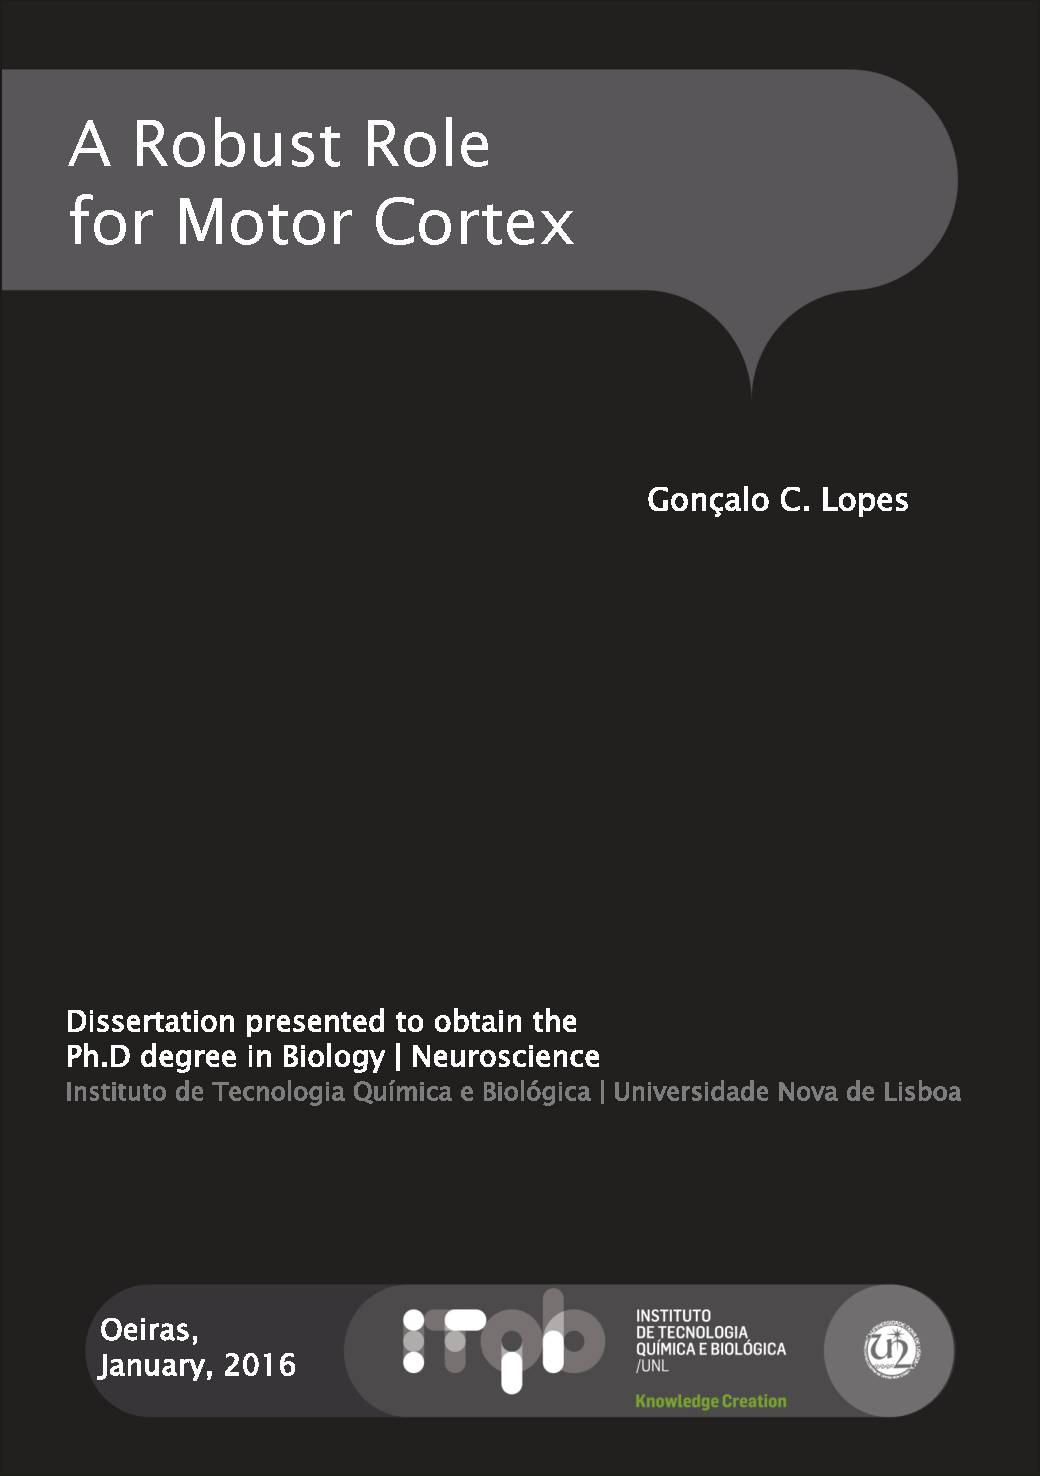
\includepdf[pages={1}]{chapters/Cover.pdf}
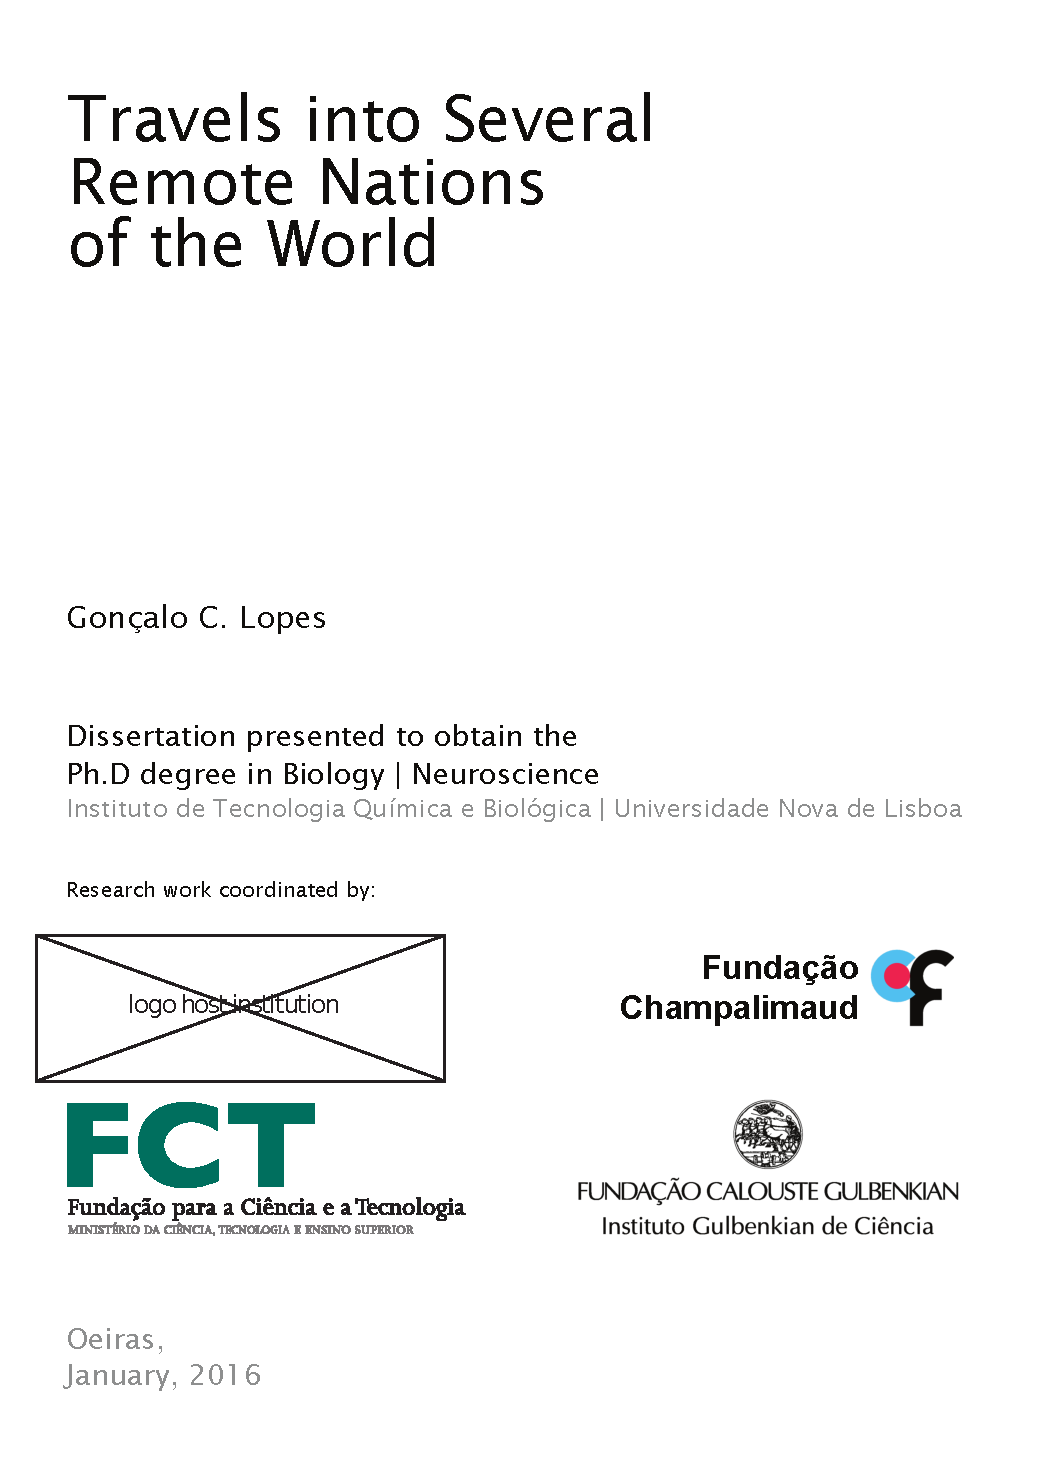
\includepdf[pages={1}]{chapters/TitlePage.pdf}

\maketitlepage
\makefrontmatter

% If you've disabled frontmatter, you can insert the toc manually
%\tableofcontents\clearpage

%%%% %%%% Import chapters
%\include lets  us split up the document (and each include starts a new page):

\chapter{Towards a Teleology of Cortical Motor Control}
\epigraph{The infinite fertility of the organism as a field for adapted reactions has become more apparent. The purpose of a reflex seems as legitimate and urgent an object for natural inquiry as the purpose of the colouring of an insect or a blossom. And the importance to physiology is, that the reflex reaction cannot be really intelligible to the physiologist until he knows its aim.}{\textsc{Sir Charles S. Sherrington}, \textit{The Integrative Action of the Nervous System} (1906)}
				
% !TEX root = ../ThesisTemplateCNP.tex
	

% Chapter summary
				
\section{Chapter Summary}

The author permitted to see the grand academy of Lagado.  The academy largely described.  The arts wherein the professors employ themselves.

\pagebreak




% Visit to Lagado
\section{Visit to the Academy of Lagado}

This academy is not an entire single building, but a continuation of several houses on both sides of a street, which growing waste, was purchased and applied to that use.


I was received very kindly by the warden, and went for many days to the academy.  Every room has in it one or more projectors; and I believe I could not be in fewer than five hundred rooms.

The first man I saw was of a meagre aspect, with sooty hands and face, his hair and beard long, ragged, and singed in several places.  His clothes, shirt, and skin, were all of the same colour.  He has been eight years upon a project for extracting sunbeams out of cucumbers, which were to be put in phials hermetically sealed, and let out to warm the air in raw inclement summers.  He told me, he did not doubt, that, in eight years more, he should be able to supply the governor’s gardens with sunshine, at a reasonable rate: but he complained that his stock was low, and entreated me “to give him something as an encouragement to ingenuity, especially since this had been a very dear season for cucumbers.”  I made him a small present, for my lord had furnished me with money on purpose, because he knew their practice of begging from all who go to see them.

I went into another chamber, but was ready to hasten back, being almost overcome with a horrible stink.  My conductor pressed me forward, conjuring me in a whisper “to give no offence, which would be highly resented;” and therefore I durst not so much as stop my nose.  The projector of this cell was the most ancient student of the academy; his face and beard were of a pale yellow; his hands and clothes daubed over with filth.  When I was presented to him, he gave me a close embrace, a compliment I could well have excused.  His employment, from his first coming into the academy, was an operation to reduce human excrement to its original food, by separating the several parts, removing the tincture which it receives from the gall, making the odour exhale, and scumming off the saliva.  He had a weekly allowance, from the society, of a vessel filled with human ordure, about the bigness of a Bristol barrel.

I saw another at work to calcine ice into gunpowder; who likewise showed me a treatise he had written concerning the malleability of fire, which he intended to publish.

There was a most ingenious architect, who had contrived a new method for building houses, by beginning at the roof, and working downward to the foundation; which he justified to me, by the like practice of those two prudent insects, the bee and the spider.

There was a man born blind, who had several apprentices in his own condition: their employment was to mix colours for painters, which their master taught them to distinguish by feeling and smelling.  It was indeed my misfortune to find them at that time not very perfect in their lessons, and the professor himself happened to be generally mistaken.  This artist is much encouraged and esteemed by the whole fraternity.

In another apartment I was highly pleased with a projector who had found a device of ploughing the ground with hogs, to save the charges of ploughs, cattle, and labour.  The method is this: in an acre of ground you bury, at six inches distance and eight deep, a quantity of acorns, dates, chestnuts, and other mast or vegetables, whereof these animals are fondest; then you drive six hundred or more of them into the field, where, in a few days, they will root up the whole ground in search of their food, and make it fit for sowing, at the same time manuring it with their dung: it is true, upon experiment, they found the charge and trouble very great, and they had little or no crop.  However it is not doubted, that this invention may be capable of great improvement.

I went into another room, where the walls and ceiling were all hung round with cobwebs, except a narrow passage for the artist to go in and out.  At my entrance, he called aloud to me, “not to disturb his webs.”  He lamented “the fatal mistake the world had been so long in, of using silkworms, while we had such plenty of domestic insects who infinitely excelled the former, because they understood how to weave, as well as spin.”  And he proposed further, “that by employing spiders, the charge of dyeing silks should be wholly saved;” whereof I was fully convinced, when he showed me a vast number of flies most beautifully coloured, wherewith he fed his spiders, assuring us “that the webs would take a tincture from them; and as he had them of all hues, he hoped to fit everybody’s fancy, as soon as he could find proper food for the flies, of certain gums, oils, and other glutinous matter, to give a strength and consistence to the threads.”

There was an astronomer, who had undertaken to place a sun-dial upon the great weathercock on the town-house, by adjusting the annual and diurnal motions of the earth and sun, so as to answer and coincide with all accidental turnings of the wind.

I was complaining of a small fit of the colic, upon which my conductor led me into a room where a great physician resided, who was famous for curing that disease, by contrary operations from the same instrument.  He had a large pair of bellows, with a long slender muzzle of ivory: this he conveyed eight inches up the anus, and drawing in the wind, he affirmed he could make the guts as lank as a dried bladder.  But when the disease was more stubborn and violent, he let in the muzzle while the bellows were full of wind, which he discharged into the body of the patient; then withdrew the instrument to replenish it, clapping his thumb strongly against the orifice of then fundament; and this being repeated three or four times, the adventitious wind would rush out, bringing the noxious along with it, (like water put into a pump), and the patient recovered.  I saw him try both experiments upon a dog, but could not discern any effect from the former.  After the latter the animal was ready to burst, and made so violent a discharge as was very offensive to me and my companion.  The dog died on the spot, and we left the doctor endeavouring to recover him, by the same operation.

I visited many other apartments, but shall not trouble my reader with all the curiosities I observed, being studious of brevity.

I had hitherto seen only one side of the academy, the other being appropriated to the advancers of speculative learning, of whom I shall say something, when I have mentioned one illustrious person more, who is called among them “the universal artist.”  He told us “he had been thirty years employing his thoughts for the improvement of human life.”  He had two large rooms full of wonderful curiosities, and fifty men at work.  Some were condensing air into a dry tangible substance, by extracting the nitre, and letting the aqueous or fluid particles percolate; others softening marble, for pillows and pin-cushions; others petrifying the hoofs of a living horse, to preserve them from foundering.  The artist himself was at that time busy upon two great designs; the first, to sow land with chaff, wherein he affirmed the true seminal virtue to be contained, as he demonstrated by several experiments, which I was not skilful enough to comprehend.  The other was, by a certain composition of gums, minerals, and vegetables, outwardly applied, to prevent the growth of wool upon two young lambs; and he hoped, in a reasonable time to propagate the breed of naked sheep, all over the kingdom.

We crossed a walk to the other part of the academy, where, as I have already said, the projectors in speculative learning resided.

The first professor I saw, was in a very large room, with forty pupils about him.  After salutation, observing me to look earnestly upon a frame, which took up the greatest part of both the length and breadth of the room, he said, “Perhaps I might wonder to see him employed in a project for improving speculative knowledge, by practical and mechanical operations.  But the world would soon be sensible of its usefulness; and he flattered himself, that a more noble, exalted thought never sprang in any other man’s head.  Every one knew how laborious the usual method is of attaining to arts and sciences; whereas, by his contrivance, the most ignorant person, at a reasonable charge, and with a little bodily labour, might write books in philosophy, poetry, politics, laws, mathematics, and theology, without the least assistance from genius or study.”  He then led me to the frame, about the sides, whereof all his pupils stood in ranks.  It was twenty feet square, placed in the middle of the room.  The superfices was composed of several bits of wood, about the bigness of a die, but some larger than others.  They were all linked together by slender wires.  These bits of wood were covered, on every square, with paper pasted on them; and on these papers were written all the words of their language, in their several moods, tenses, and declensions; but without any order.  The professor then desired me “to observe; for he was going to set his engine at work.”  The pupils, at his command, took each of them hold of an iron handle, whereof there were forty fixed round the edges of the frame; and giving them a sudden turn, the whole disposition of the words was entirely changed.  He then commanded six-and-thirty of the lads, to read the several lines softly, as they appeared upon the frame; and where they found three or four words together that might make part of a sentence, they dictated to the four remaining boys, who were scribes.  This work was repeated three or four times, and at every turn, the engine was so contrived, that the words shifted into new places, as the square bits of wood moved upside down.


Six hours a day the young students were employed in this labour; and the professor showed me several volumes in large folio, already collected, of broken sentences, which he intended to piece together, and out of those rich materials, to give the world a complete body of all arts and sciences; which, however, might be still improved, and much expedited, if the public would raise a fund for making and employing five hundred such frames in Lagado, and oblige the managers to contribute in common their several collections.

He assured me “that this invention had employed all his thoughts from his youth; that he had emptied the whole vocabulary into his frame, and made the strictest computation of the general proportion there is in books between the numbers of particles, nouns, and verbs, and other parts of speech.”

I made my humblest acknowledgment to this illustrious person, for his great communicativeness; and promised, “if ever I had the good fortune to return to my native country, that I would do him justice, as the sole inventor of this wonderful machine;” the form and contrivance of which I desired leave to delineate on paper, as in the figure here annexed.  I told him, “although it were the custom of our learned in Europe to steal inventions from each other, who had thereby at least this advantage, that it became a controversy which was the right owner; yet I would take such caution, that he should have the honour entire, without a rival.”

We next went to the school of languages, where three professors sat in consultation upon improving that of their own country.

The first project was, to shorten discourse, by cutting polysyllables into one, and leaving out verbs and participles, because, in reality, all things imaginable are but norms.

The other project was, a scheme for entirely abolishing all words whatsoever; and this was urged as a great advantage in point of health, as well as brevity.  For it is plain, that every word we speak is, in some degree, a diminution of our lunge by corrosion, and, consequently, contributes to the shortening of our lives.  An expedient was therefore offered, “that since words are only names for things, it would be more convenient for all men to carry about them such things as were necessary to express a particular business they are to discourse on.”  And this invention would certainly have taken place, to the great ease as well as health of the subject, if the women, in conjunction with the vulgar and illiterate, had not threatened to raise a rebellion unless they might be allowed the liberty to speak with their tongues, after the manner of their forefathers; such constant irreconcilable enemies to science are the common people.  However, many of the most learned and wise adhere to the new scheme of expressing themselves by things; which has only this inconvenience attending it, that if a man’s business be very great, and of various kinds, he must be obliged, in proportion, to carry a greater bundle of things upon his back, unless he can afford one or two strong servants to attend him.  I have often beheld two of those sages almost sinking under the weight of their packs, like pedlars among us, who, when they met in the street, would lay down their loads, open their sacks, and hold conversation for an hour together; then put up their implements, help each other to resume their burdens, and take their leave.

But for short conversations, a man may carry implements in his pockets, and under his arms, enough to supply him; and in his house, he cannot be at a loss.  Therefore the room where company meet who practise this art, is full of all things, ready at hand, requisite to furnish matter for this kind of artificial converse.

Another great advantage proposed by this invention was, that it would serve as a universal language, to be understood in all civilised nations, whose goods and utensils are generally of the same kind, or nearly resembling, so that their uses might easily be comprehended.  And thus ambassadors would be qualified to treat with foreign princes, or ministers of state, to whose tongues they were utter strangers.

I was at the mathematical school, where the master taught his pupils after a method scarce imaginable to us in Europe.  The proposition, and demonstration, were fairly written on a thin wafer, with ink composed of a cephalic tincture.  This, the student was to swallow upon a fasting stomach, and for three days following, eat nothing but bread and water.  As the wafer digested, the tincture mounted to his brain, bearing the proposition along with it.  But the success has not hitherto been answerable, partly by some error in the quantum or composition, and partly by the perverseness of lads, to whom this bolus is so nauseous, that they generally steal aside, and discharge it upwards, before it can operate; neither have they been yet persuaded to use so long an abstinence, as the prescription requires.





\chapter{Neurotechnology for Behaviour}
\epigraph{It is not true that ``the laboratory can never be like life.'' The laboratory \emph{must} be like life!}{\textsc{James J. Gibson}, \textit{The Ecological Approach to Visual Perception} (1979)}
				
% !TEX root = ../ThesisTemplateCNP.tex
	

% Chapter summary
				
\section{Chapter Summary}

The design of modern scientific experiments requires the control and monitoring of many different data streams. However, the serial execution of programming instructions in a computer makes it a challenge to develop software that can deal with the asynchronous, parallel nature of scientific data. Here we present Bonsai, a modular, high-performance, open-source visual programming framework for the acquisition and online processing of data streams. We describe Bonsai's core principles and architecture and demonstrate how it allows for the rapid and flexible prototyping of integrated experimental designs in neuroscience. We specifically highlight some applications that require the combination of many different hardware and software components, including video tracking of behavior, electrophysiology and closed-loop control of stimulation.

\pagebreak




% Modular Box
				
\section{Introduction}

The formal study of animal behaviour has a long history spanning hundreds of years across the fields of ethology, experimental psychology and neuroscience. While the ethologists mainly endeavoured to study behaviour in its natural environment, the psychologists and neurophysiologists have classically resorted, of necessity, to more controlled laboratory settings. The reason is mainly one of complexity. Behaviour is a highly multi-dimensional, multi-scale phenomenon that often allows no clear separation between relevant and irrelevant variables \cite{Gomez-Marin2014}. It is in general impossible to predict what an animal is going to do simply because some of the crucial information is not even accessible to measurement. In order to mitigate this problem, neuroscientists resort to making impoverished preparations where the number of variables that are changing at any given moment is low and very carefully controlled. The hope is that in this way the interpretation of brain signals recorded simultaneously with animal behaviour will be facilitated.

Depending on the kind of question a neuroscientist is after, an appropriate behaviour paradigm is set up. Anaesthetized and head-fixed preparations, as well as classical or operant conditioning boxes are regularly employed to drive the behaviour of the animal to oscillate between a set of repeatedly reproducible states more amenable to statistical analysis. Building such behaviour assays often requires very specialized engineering skills and long development cycles of trial and error in order to ensure all the relevant variables are controlled accordingly. Because of this, the tendency of the field has been to concentrate on a small set of ``standardized'' assays which have been shown to work for one area of research or other. Small variations to the standard tasks are gradually introduced in order to probe different aspects of the system. The complexity of behaviour studies in neuroscience has thus traditionally progressed by attrition and painstaking accumulation of small perturbations to overall design patterns.

Interestingly, however, many of the most significant conceptual advances in our understanding of brain function have in fact developed \emph{pari passu} with forays into entirely new behaviour spaces. Moving from anaesthetized to awake physiology completely changed the way we understand the neural processing of sensory stimuli \cite{Sellers2015}. Similarly, moving from head-fixed to freely moving behaviour led to the discovery of place fields in hippocampus \cite{OKeefe1971}. Single trial analysis of simultaneously recorded responses have revealed patterns of neural activity such as hippocampal ripples that are simply impossible to recover from statistical averages of repetitive behaviour episodes \cite{Foster2006,Davidson2009}. Each of these developments has required significant advances in tools used to record and control behavioural data at a fine scale. Unfortunately, the technical cost and scientific risk of trying something novel means that such advances are still much fewer and far between than would be desirable.

From the beginning of this work it was understood that revealing the teleology of cortical control over behaviour would require just this kind of foray into diverse and potentially unknown behaviour spaces. We agreed that it might be worth to try and develop a toolkit for the behavioural neuroscientist that would accelerate the exploration of this vast space. One of the first obvious targets for improvement was the behaviour box. Traditionally, when a given behaviour assay is found to produce interesting results, its design is progressively tweaked so as to exacerbate the features of the original effect. In this work, we started by breaking apart this concept of the polished behaviour box, and wondered what would happen if instead of a standard box, we could have a box of standards.

\section{The Modular Behaviour Box}

At the outset it was decided that the scale of the modular architecture would probably have to match a given animal model, given the vastly different size scales between rodents, cats and primates. Our animal model of choice is the rodent \emph{rattus norvegicus}, and all of our proposed design choices target its size scale. Small adjustments could, however, be reasonably made up to a point for other mammals of similar stature, such as mice.

The main component and interface of the modular box is the individual $1\times 1$ module (Figure \ref{fig:modules}A). This module defines a standardized footprint ($\SI{12}{\centi\meter}\times \SI{12}{\centi\meter}$), against which all other modules are measured. Every newly fabricated module is built to specification to match a multiple of this standardized footprint (e.g. it is possible to have $2\times 1$, $2\times 2$, $4\times 1$ or any other multiple combination of the standard size). Inside the module footprint the module designer places a single logical component of a behaviour box and ensures that it can operate in isolation. Figure \ref{fig:modules} shows some examples of reusable modules developed throughout the project.

\begin{figure}
\centering
\includestandalone[scale=1.00]{chapters/figuresChTools/modules}
\caption{Some examples of standardized behaviour modules. (\textbf{A}) Detail of a $1\times 1$ module mounted in support frame. Fixation is achieved by driving a screw through post-insertion nuts placed in the structural framing (see text). (\textbf{B}) Example reward port module which can be floor- or wall-mounted. All relevant electronics and water distribution circuits are assembled on the back of the module (not shown). (\textbf{C}) Wall-mounted reconfigurable obstacle course stepper module. Stepper motors mounted on the back of the module allow for dynamic reconfiguration of the orientation of each step. (\textbf{D}) Floor-mounted obstacle course step pair. Multiple of these modules can be tiled together to assemble obstacle courses of arbitrary length.}
\label{fig:modules}
\end{figure}

\begin{figure}
\centering
\includestandalone[scale=1.00]{chapters/figuresChTools/box}
\caption{Example of a linear shuttling box assembled from a $\SI{1}{\meter}\times \SI{1}{\meter}$ modular structure using reward port and obstacle course step modules.}
\label{fig:box}
\end{figure}

\begin{figure}
\centering
\includestandalone[scale=0.90]{chapters/figuresChTools/box3d}
\caption{Side view of the linear shuttling box.}
\label{fig:box3d}
\end{figure}

\begin{figure}
\centering
\includestandalone[scale=1.00]{chapters/figuresChTools/verticalBox}
\caption{Example of vertical assembly. (\textbf{A}) Detail of a $1\times 1$ wall-mounted platform module. (\textbf{B}) Example of a vertical maze configuration.}
\label{fig:verticalBox}
\end{figure}

One of the principal requirements for assembling a box is fastening all its components together. By having a standard footprint, it is possible to design a set of regularly spaced mounting points that allows the experimentalist to quickly generate an entirely new configuration by simply swapping modular components inside the box (Figure \ref{fig:box}, \ref{fig:box3d}). For this work, we took advantage of an existing aluminium structural framing system (Bosch Rexroth, DE) to build the common mounting points (Figure \ref{fig:modules}A). Modules are fastened against post-insertion nuts which are able to slide across the whole length of the aluminium rail. Each of the modules is fastened by four screws, one in each corner. In order to ensure modules can be tightly and securely fixed one next to the other, we used a system of regularly spaced double rails (Figure \ref{fig:box}). This gives the frame the flexibility to easily reposition and rearrange individual modules tiling the entire footprint of any arbitrarily large box.

If the support frame is laid out vertically, it is possible to create modular walls of arbitrary dimensions. Some of the modules can be mounted equally well on a vertical or horizontal configuration, such as reward ports (Figure \ref{fig:modules}B). The three-dimensionality of the design has even been exploited to create vertical mazes (Figure \ref{fig:verticalBox}) to great success.

Throughout the project we made the base of every module from \SI{5}{\milli\meter} acrylic pieces. While not an absolute requirement for the design, this choice of plastic material has the advantage that a laser cutter can be used to very quickly produce a large collection of custom-built modules. In addition, patterns can be engraved or cut on the base to provide additional mounting points for hardware embedded in the module. The use of such rapid prototyping fabrication tools alongside with off the shelf available electronic sensors and actuators meant we were able to completely redesign the entire behaviour box, sometimes in a matter of days.


% Bonsai
				
\section{Rapid Prototyping of Behaviour Experiments}

Modern scientific experiments crucially depend on the control and monitoring of many parallel streams of data. Multiple measurement devices, from video cameras, microphones, and pressure sensors to neural electrodes, must simultaneously send their data in real-time to a recording system. General purpose digital computers have gradually replaced many of the specialized analog and digital technologies used for this kind of data acquisition and experiment control, largely due to the flexibility of programming and the exponential growth in computing power. However, the serial nature of programming instructions and shared memory makes it a challenge, even for experienced programmers, to develop software that can elegantly deal with the asynchronous, parallel nature of scientific data.

Another challenge arises from the need for software integration. Each hardware vendor provides their own set of drivers and programming interfaces for configuring and acquiring data from their devices. In addition, the growth of the open-source movement has greatly increased the number of freely available technologies for different data processing domains. Integration of these diverse software and hardware components remains a major challenge for researchers.

These difficulties lead to increased development times when setting up an experiment. Moreover, it requires experimenters to pursue specialized training outside their domain of research. This limits the ability to rapidly prototype and try out new designs and can quickly become the factor limiting the kinds of questions that are amenable to scientific investigation.

Here we describe Bonsai, an open-source visual programming framework for processing data streams. The main goal of Bonsai is to simplify and accelerate the development of software for acquiring and processing the many heterogeneous data sources commonly used in (neuro) scientific research. We aim to facilitate the fast implementation of state-of-the-art experimental designs and to encourage the exploration of new paradigms. The framework has already been successfully used for many applications. In the following we will specifically highlight Bonsai's utility in neuroscience for monitoring and controlling a diverse range of behaviour and physiology experiments.

\subsection{Getting Started with Bonsai}

\subsubsection{Community}

The Bonsai framework can be downloaded at \url{https://bitbucket.org/horizongir/bonsai} and installed on Windows operating systems starting with Windows 7 and above. The website is organized into different sections: Downloads (where the latest installer is located), Wiki (with a “Getting Started” guide, tutorials and (FAQ) frequently asked questions), and Issues (where bugs can be reported). We have also created a user forum (address is listed in the FAQ section) where the community of Bonsai users have been sharing their feedback, questions and experiences.

A video tutorial introduction to Bonsai is included with this publication (Supplementary Video 1).

\subsubsection{Extending Bonsai}

Bonsai was designed from the outset to support many different layers of extensibility:
\begin{enumerate}[(a)]
    \item Dataflows: The first layer is through the creation of Bonsai dataflow files themselves. Existing dataflows can be directly reused inside other dataflows as nested nodes. This allows for the sharing of reusable dataflow design patterns between applications.
    \item Python Scripting: Bonsai supports embedded scripting using IronPython 2.7. Specifically, Bonsai includes three types of Python nodes: PythonTransform, PythonCondition, and PythonSink, which all operate by calling a user-defined Python function described by a script. Below we include a simple example of a PythonTransform for rescaling data:

    \begin{lstlisting}[language=Python]
# Declare transform output type
@returns(float)
def process(value):
    return value / 255.0
    \end{lstlisting}

    \item NuGet: Bonsai modules are natively written in C\# or other.NET languages. The NuGet package manager has emerged as the defacto standard for the sharing of code between.NET developers. Bonsai includes a full NuGet client which manages local package versions, provides access to the curated feed of standard Bonsai packages, and allows for the quick sharing of modules between Bonsai users through either NuGet or other remote and local package sources. Tutorials and examples on how to create new Bonsai modules are included in the Wiki.
\end{enumerate}

\subsection{Architecture}

Scientific data, like the world we live in, is inherently parallel. To monitor this complexity, modern experimenters are often forced to use multiple electronic instruments simultaneously, each with their own independent sampling rates. As data arrives at the acquisition computer, there are two main approaches to log and process these asynchronous data streams. The first approach is to use a polling strategy: a single sequential process in the computer runs a processing loop that goes through each device in sequence and gathers the available data. In this case, data from only one device is being collected and manipulated at any point in time. The second approach is to use an event-driven (reactive) architecture: processes are setup in parallel to collect data from all the devices simultaneously. Whenever new data is available, notifications are sent to the appropriate software routines that collect and process the data as soon as possible. When only a single processor is available, the difference between these two strategies is negligible: only one instruction at a time can be executed by the computer. However, with modern multi-processor cores and dedicated data transfer circuits, the performance difference between the two approaches will significantly influence the throughput of a data acquisition and processing system. Unfortunately, software tools to support and facilitate the “reactive” approach to data stream processing are only just now starting to be adopted and most software systems are still built from the sequential composition of simple program routines. Many of the assumptions of the sequential processing scenario do not scale to handle parallel execution, especially when shared memory and resources are involved.

In recent years, a number of advances in programming languages and software frameworks have tried to make it easier to create complex software applications by composition of asynchronous computing elements \cite{Bainomugisha2013}. Bonsai builds upon these new efforts and aims to extend these developments to the rapid-prototyping domain by introducing a visual programming language for composing and processing asynchronous data streams. Bonsai was developed on top of the Reactive Extensions for the.NET framework (Rx) \cite{MicrosoftOpenTechnologies2014}. Rx provides many built-in operators that transparently deal with the concurrency challenges that inevitably surface when multiple data streams need to be processed and integrated together in a single program. It has become an increasingly popular framework to develop reactive interfaces for next generation mobile and desktop computing platforms, where it is used to handle the growing number of sensors and network communications required by business logic and consumer applications.

Bonsai (via Rx) represents asynchronous data streams using the notion of an observable sequence. An observable sequence represents a data stream where elements follow one after the other. An example would be a sequence of frames being captured by a camera, or a sequence of key presses logged by the keyboard. The name observable simply specifies that the way we access elements in the data stream is by listening to (i.e., observing) the data as it arrives, in contrast with the static database model, in which the desired data is enumerated.

In Bonsai, observable sequences are created and manipulated graphically using a dataflow \cite{Mosconi2000, Johnston2004} representation (Figures \ref{fig:bonsaiInterface}, \ref{fig:bonsaiExamples}A, Supplementary Video 1). Each node in the dataflow represents an observable sequence. Nodes can be classified as either observable sources of data or combinators (Table \ref{tab:bonsaiCategories}). Sources deliver access to raw data streams, such as images from a video camera or signal waveforms from a microphone or electrophysiology amplifier. Combinators represent any observable operator that handles one or more of these sequences. This category can be further specialized into transforms, sinks and other operator types depending on how they manipulate their inputs (Table \ref{tab:bonsaiCategories}). Transforms modify the incoming data elements of a single input sequence. An example would be taking a sequence of numbers and generating another sequence of numbers containing the original elements multiplied by two. Sinks, on the other hand, simply introduce processing side-effects without modifying the original sequence at all. One example would be printing each number in the sequence to a text file. The act of printing in itself changes nothing about the sequence, which continues to output every number, but the side-effect will generate some useful action. Combinators that change, filter or merge the flow of data streams are neither transforms nor sinks, and they are simply referred to by the more general term combinator. The Sample combinator illustrated in Figure \ref{fig:bonsaiExamples}A takes two data sequences and produces a new sequence where elements are sampled from the first sequence whenever the second sequence produces a new value. In this example, we use Sample to extract and save single images from a video stream whenever a key is pressed.

\begin{figure}
\begin{center}
\scalebox{0.7}{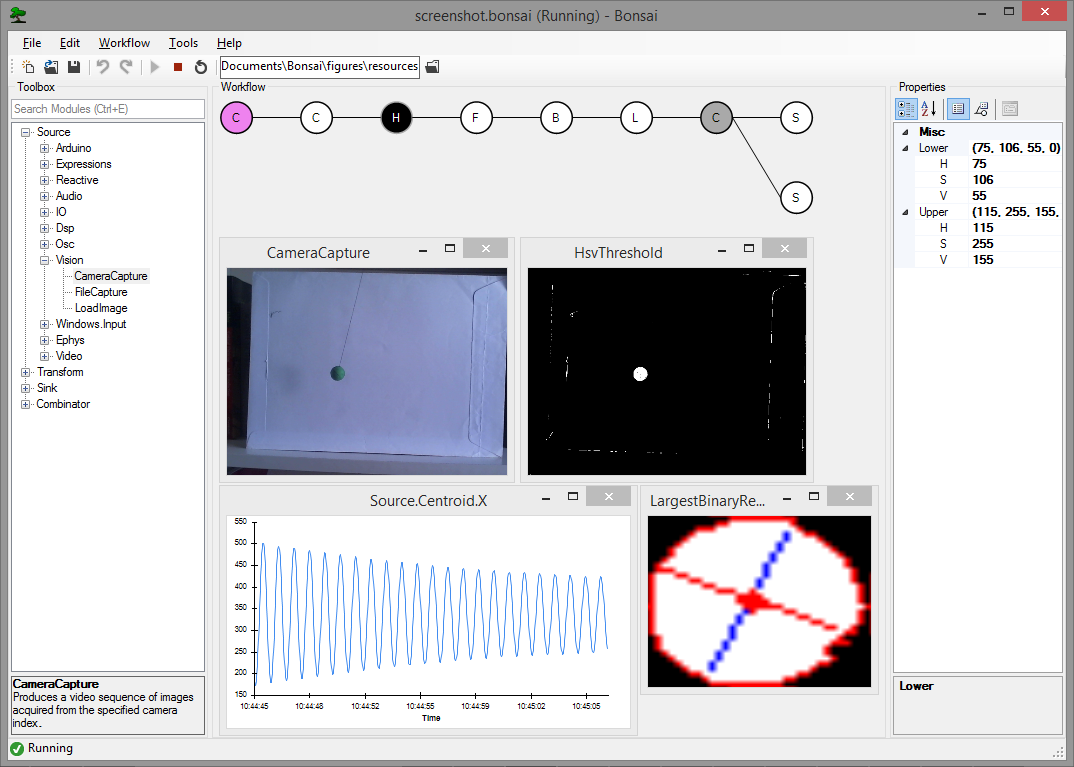
\includegraphics[width=\linewidth]{chapters/figuresChTools/bonsaiInterface.png}}
\end{center}
\vspace{-5mm}
\caption{Screenshot of the Bonsai user interface running a video processing pipeline. An example dataflow for color segmentation and tracking of a moving pendulum is shown. Data sources are colored in violet; transform operators in white; sinks in dark gray. The currently selected node (HsvThreshold) is colored in black and its configuration parameters are displayed in the properties panel on the right. Overlaid windows and graphs represent Bonsai data visualizers for the output of individual nodes.}
\label{fig:bonsaiInterface}
\end{figure}

\begin{figure}
\begin{center}
\scalebox{0.5}{\includesvg{chapters/figuresChTools/bonsaiExamples}}
\end{center}
\vspace{-5mm}
\caption{Examples of dataflow processing pipelines using Bonsai. \textbf{(A)} Taking grayscale snapshots from a camera whenever a key is pressed. Top: graphical representation of the Bonsai dataflow for camera and keyboard processing. Data sources are colored in violet; transform operators in white; combinators in light blue; sinks in dark gray. Bottom: marble diagram showing an example execution of the dataflow. Colored tokens represent frames arriving from the camera. Black circles represent key press events from the keyboard. Asterisks indicate saving of images to permanent storage. \textbf{(B)} Dynamic modulation of an image processing threshold using the mouse. The x-coordinate of mouse movements is used to directly set the externalized ThresholdValue property (orange). The updated threshold value will be used to process any new incoming images. \textbf{(C)} Grouping a set of complex transformations into a single node. In the nested dataflow, the source represents incoming connections to the group and the sink represents the group output.}
\label{fig:bonsaiExamples}
\end{figure}

\begin{table}
\begin{center}
\scalebox{0.7}{\includesvg{chapters/figuresChTools/bonsaiCategories}}
\end{center}
\vspace{-5mm}
\caption{List of Bonsai node categories. The color of each Bonsai node serves as a visual aid to identify their role in dataflow processing pipelines. Most of these categories are actually specializations of the very general combinator and are meant to visually depict their specific data processing semantics.}
\label{tab:bonsaiCategories}
\end{table}

A common requirement when designing and manipulating dataflows is the ability to visualize the state of the data at different stages of processing. We have therefore included a set of visualizers to assist debugging and inspection of data elements, including images and signal waveforms (Figure \ref{fig:bonsaiInterface}). These visualizers are automatically associated with the output data type of each node and can be launched at any time in parallel with the execution of the dataflow. Furthermore, it is often desirable to be able to manipulate processing parameters online for calibration purposes. Each node has a set of properties which parameterize the operation of that particular source or combinator (Figure \ref{fig:bonsaiInterface}). This allows, for example, changing the cutoff frequency of a signal processing filter, or setting the name of the output file in the case of data recording sinks. We have also included the possibility of externalizing node properties into the dataflow (Figure \ref{fig:bonsaiExamples}B). Externalizing a property means extracting one of the parameters into its own node in the dataflow, making it possible to connect the output of another node to the exposed property. This allows for the dynamic control of node parameters.

Finally, we have built into Bonsai the ability to group nodes hierarchically. In its simplest form, this feature can be used to encapsulate a set of operations into a single node which can be reused elsewhere (Figure \ref{fig:bonsaiExamples}C). This is similar to defining a function in a programming language and is one of the ways to create new reactive operators in Bonsai. Any named externalized properties placed inside an encapsulated dataflow will also show up as properties of the group node itself. This allows for the parameterization of nested dataflows and increases their reuse possibilities. In addition, encapsulated dataflows are used to specify more complicated, yet powerful, operators such as iteration constructs that allow for the compact description of complex data processing scenarios that can be cumbersome to specify in pure dataflow visual languages \cite{Mosconi2000} (see below).

Bonsai was designed to be a modular framework, which means it is possible to extend its functionality by installing additional packages containing sources and combinators developed for specific purposes. New packages can be written using C\# or any of the.NET programming languages. Python scripts [via IronPython \cite{IronPython2014}] can be embedded in the dataflow as transforms and sinks, allowing for rapid integration of custom code. All functionality included in Bonsai was designed using these modular principles, and we hope to encourage other researchers to contribute their own packages and thereby extend the framework to other application domains. At present, the available packages include computer vision and signal processing modules based on the OpenCV library \cite{Itseez2014}. Drivers for several cameras and interfaces to other imaging and signal acquisition hardware were integrated as Bonsai sources and sinks, including support for Arduino microcontrollers \cite{Banzi2014}, serial port devices and basic networking using the OSC protocol \cite{Wright2003}. Given the specific applications in the domain of neuroscience, we also integrated a number of neuroscience technology packages. The Ephys package, for example, builds on the Open Ephys initiative for the sharing of electrophysiology acquisition hardware \cite{Voigts2013} by providing support for the Rhythm open-source USB/FPGA interface (Intan Technologies, US). Therefore, the next generation tools for electrophysiology can already be used inside Bonsai, the acquired physiology data implicitly integrated with other available data streams and thus easily assembled into a powerful and flexible experimental neuroscience platform.

\subsection{Advanced Operators}

The most common application of Bonsai is the acquisition and processing of simple, independent data streams. However, for many modern experiments, basic acquisition and storage of data is often not sufficient. For example, it can be convenient to only record the data aligned on events of interest, such as the onset of specific stimuli. Furthermore, neuroscience experiments often progress through several stages, especially for behavioral assays, where controlled conditions vary systematically across different sessions or trials. In order to enforce these conditions, experiments need to keep track of which stage is active and use that information to update the state of control variables and sensory processing. These requirements often cannot be described by a simple linear pipeline of data, and require custom code to handle the complicated logic and bookkeeping of experimental states. Below we describe a set of advanced Bonsai operators that can be used to flexibly reconfigure data processing logic to cover a larger number of scenarios. These operators and their applications are all built on the single idea of slicing a data stream into sub-sequences, called windows, which are then processed independently and, potentially, in parallel (Figure \ref{fig:bonsaiAdvanced}).

\begin{figure}
\begin{center}
\scalebox{0.5}{\includesvg{chapters/figuresChTools/bonsaiAdvanced}}
\end{center}
\vspace{-5mm}
\caption{Using slicing and window processing combinators in Bonsai.}
\label{fig:bonsaiAdvanced}
\end{figure}

Bonsai provides different combinators that allow the creation of these sub-sequences from any observable data stream, using element count information, timing, or external triggers (Figures \ref{fig:bonsaiAdvanced}A–C). The specific set of operations to apply on each window is described by encapsulating a dataflow inside a SelectMany group, as detailed in the signal processing example of Figure \ref{fig:bonsaiAdvanced}D. The input source in this group represents each of the window sub-sequences, i.e., it is as if each of the windows is a new data source, containing only the elements that are a part of that window. These elements will be processed as soon as they are available by the encapsulated dataflow. Windows can have overlapping common elements, in which case their processing will happen concurrently. The processing outputs from each window are merged together to produce the final result. In the case of Figure \ref{fig:bonsaiAdvanced}D, past and future samples are grouped in windows to compute a running average of the signal through time, necessarily time-shifted by the number of future samples that are considered in the average.

The processing of the elements of each window happens independently, as if there was a new isolated dataflow running for each of the sequences. We can exploit this independence in order to dynamically turn dataflows on and off during an experiment. In the video splitting example of Figure \ref{fig:bonsaiAdvanced}E, we use an external trigger source to chop a continuous video stream into many small video sequences, aligned when the trigger fired. We then nest a VideoWriter sink into the SelectMany group. The VideoWriter sink is used to encode video frames into a continuous movie file. It starts by creating the video file upon arrival of the first frame, and then encoding every frame in the sequence as they arrive. When the data stream is completed, the file is closed. By nesting the VideoWriter inside the SelectMany group, what we have effectively done is to create a new video file for each of the created windows. Whenever a new trigger arrives, a new clip is created and saving proceeds, implicitly parallelized, for that video file.

More generally, we can use this idea to implement discrete transitions between different processing modes, and chain these states together to design complex control structures such as finite state machines (FSMs). FSMs are widely used to model environments and behavioral assays in systems and cognitive neuroscience. One example is illustrated in Figure \ref{fig:bonsaiAdvanced}F, where we depict the control scheme of a stimulus-response apparatus for a simple reaction time task. In this task, there are only two states: Ready and Go. In the Ready state, no stimulus is presented and a timer is armed. Whenever the timer fires, the task transitions into the Go state, and a stimulus is presented. The subject is instructed to press a key as fast as possible upon presentation of the stimulus. As soon as the key is pressed, the system goes back to the Ready state to start another trial. In a FSM, nodes represent states, e.g., stimulus availability or reward delivery, and edges represent transitions between states that are caused by events in the assay, e.g., a key press. In each state, a number of output variables and control parameters are set (e.g., turning on a light) which represent the behaviour of the machine in that state.

In the Bonsai dataflow model, dataflows encapsulated in a SelectMany group can be used to represent states in a FSM (Figure \ref{fig:bonsaiAdvanced}F, bottom). Specifically, a state is activated whenever it receives an input event, i.e., the dataflow nested inside the state will be turned on. The dynamics of the nested dataflow determine the dynamics of the state. In the Go state presented in Figure \ref{fig:bonsaiAdvanced}F, the activation event is used to trigger stimulus onset. In parallel, we start listening for the key press which will terminate the state. Conversely, for the Ready state we would trigger stimulus offset and arm the timer for presenting the next stimulus. An important difference between Bonsai dataflows and pure state machine models is that a dataflow is specified as a directed acyclic graph, i.e., the data stream cannot loop back on itself. However, by taking advantage of the Repeat combinator, we can restart a dataflow once it is completed, allowing us to reset the state machine for the next trial.

Many of the control tasks in experiments have this sequential trial-based structure, which has allowed us to rapidly prototype complex behaviour assays, such as closed-loop rodent decision making tasks, simply by leveraging the flexibility of the data stream slicing operators.

\subsection{Under the Hood}

\subsubsection{Computational Overhead}

Bonsai takes full advantage of the flexibility of C\# and its Just-In-Time (JIT) compiler to bring the computational overhead of running the framework to zero. This is possible due to the fact that the graphical dataflows in Bonsai are actually specifying syntactically correct C\# code by means of an expression tree. When the dataflow is executed, C\# code is generated for assembling and running the pipeline. This code is ultimately compiled into native machine language before execution, which has the consequence that running a Bonsai dataflow is as fast as if one wrote the equivalent Rx code manually. In fact, this also means every Bonsai module is just a standard C\# class exposing methods working on Rx's observable interface, which makes it possible to reference every single Bonsai package from a standard.NET application and just use the module functionality directly.

\subsubsection{Concurrency}

The level of concurrency and parallelism in Bonsai entirely depends on the structure of each individual dataflow and the specific computer hardware involved. Typically, each hardware device source (e.g., a camera) runs independently in its own logical thread. Some sources can occasionally share threads when the underlying device architecture allows for it. For example microcontroller sources coming from the same USB port effectively require sharing a single communications channel, but this is logically abstracted from the developer so there is no need to worry about handling multiplexed messages.

The specialized handling of concurrency introduced by merging different processing streams is done using dedicated Rx concurrency operators that are exposed graphically through the language. Operators located downstream from the merge point can treat the merged sequence as if it was a single sequential data source. This means most Bonsai operators are actually concurrency-agnostic, meaning they don't have to worry about concurrency at all: they simply assume their inputs are processed sequentially. This functional approach allows Bonsai operators to be simple to program, reliable and extremely performant.

Finally, some Bonsai operators introduce local concurrency implicitly to maximize performance. For example, many of the data logging sinks actually write to disk in parallel with the arrival of data. This prevents processor-heavy routines, such as video compression, to stall the pipeline and allow for online execution to proceed as fast as possible. From the point of view of the developer, however, such optimizations happen transparently.

\subsubsection{Time}

Being a fully asynchronous framework, Bonsai has to deal with code executing logically in many different processors. There is no particular assumption about time in the framework other than the sequential flow of data through the pipeline, but facilities are in place to help the synchronization and timing of data. For example, the Timestamp operator provides access to hardware performance timers included in modern processors to timestamp event notifications, across the pipeline, using a shared high resolution clock. However, it should be noted that this only applies to processes occurring centrally: for precise sub-millisecond synchronization of physical events happening outside the computer (e.g., stimulation pulse train and electrophysiology data) we still recommend the classical sharing of voltage or optical sync pulses logged simultaneously in each device.

\subsection{Alternatives to Bonsai}

Although graphical user interfaces have played a crucial role in the widespread proliferation of computing technology throughout various scientific fields, the majority of these interfaces tend to be applied to relatively narrow domains, such as the operation of a specific instrument. Their goal is often to provide access to all the various configuration parameters of the hardware and to provide basic data acquisition functionality. There is often no opportunity to parameterize or condition the behaviour of the instrument beyond the possibilities presented by the interface, and interconnections with other devices are often limited to simple hardware triggers. The alternative, when available, is to access low-level application programming interfaces (APIs), and program the desired behaviour from scratch.

In the more flexible domains of data analysis, behaviour control and software simulations, the use of more versatile graphical interfaces has become increasingly prevalent. In these scenarios, it is not uncommon to encounter the development of domain-specific languages (DSLs), where graphical building blocks related to the domain of application can be combined together by the user to generate new behaviors, such as the sequence of steps in a psychophysics experiment or a state-machine diagram used to control stimuli and rewards in operant conditioning. While providing more flexibility to the end user, such DSLs are usually not conceived, at their core, to be applied to wildly different domains (e.g., an operant conditioning state machine is not expected to be able to filter continuous electrophysiology signals). In fact, most DSLs will not even allow the user to extend the set of built-in operations. In those that do, the developer may find a customization pit \cite{Cook2007}, where concepts and operations that are within the range of what the DSL can express are easy to develop, whereas tasks that are a little bit outside of the boundaries of the language quickly become impossible or too cumbersome to implement.

As the level of flexibility of a graphical user interface increases, we start to approach the space occupied by general purpose visual programming languages (GPVPL). These are languages that are designed from the outset to be capable of solving problems across a wide variety of domains using a general set of operations. Ideally, the core building blocks of the language will themselves be domain-independent, so that the user can easily apply the same set of operations to the widest possible class of inputs. In order to better illustrate the feel and expressive power of GPVPLs, and to clarify where Bonsai itself is positioned, we will give two examples of popular languages that have succeeded in this niche: LabVIEW \cite{Instruments2014} and Simulink \cite{MathWorks2014}.

LabVIEW is one of the best examples of a GPVPL applied to the design and control of experiments \cite{Elliott2007}. In LabVIEW, users create virtual instruments (VIs) which are composed of a graphical front-panel containing an assortment of buttons, dials, charts and other objects; as well as a back-panel where a flowchart-like block diagram can be used to specify the behaviour of the VI. In this back-panel, nodes and terminal elements can represent hardware components, numerical operations or front-panel objects, which are connected together using virtual wires that specify the flow of data between them. The popularity of LabVIEW grew initially from its support for state-of-the-art data acquisition cards and hardware as well as its data visualization capabilities. The modularity of its architecture also allowed users to quickly develop and implement new nodes within the language itself by using VIs themselves as nodes.

Although the LabVIEW back-panel is a dataflow visual programming language, its execution model tends to follow a polling, rather than event-driven, strategy for dealing with multiple data streams. In order to properly scale this model to the increasing number of available processor cores, LabVIEW has implemented sophisticated code analysis tools that attempt to identify parallelizable portions of block diagrams automatically (Elliott et al., 2007). Once these sections are identified, LabVIEW will automatically generate parallel processes depending on the number of available cores and will manage the bottlenecks in the code accordingly. Although this mitigates the limitations of the sequential polling programming model, it is important to realize that the goal of such automatic parallelization is still to provide the user with a logically synchronized programming model.

Simulink is a popular dataflow visual programming language for modeling, simulating and analyzing multi-domain dynamic systems. It has become extremely popular for modeling response characteristics of control systems, allowing not only for the rapid prototyping of algorithms, but also the automatic generation of microcontroller code for embedded systems. Again, the success of the language stemmed primarily from the flexibility and ease of use of the block diagrams, as well as the number of prebuilt operations and data visualization tools which quickly took care of many crucial but tedious aspects of control systems modeling.

Like LabVIEW, the execution model for Simulink generated code is still based on polling strategies, where ready to execute dataflow nodes are updated in turn as inputs become available. Again, strategies to scale the output of Simulink to multiple cores have been proposed based on analyzing and segmenting the model into parallelizable sections which can be converted into equivalent parallel execution code for microcontrollers \cite{Kumura2012}.

Similar to LabVIEW and Simulink, Bonsai was designed as a general purpose modular language. The core architecture of Bonsai is domain-independent and provides a general framework to compose asynchronous data streams. A general set of composition operators, or combinators, provides support for iteration, segmentation and merging of parallel data streams, as well as other common manipulations on observable sequences. Both the sources of data and available processing operations can be extended within the language itself using nesting of dataflows. Data visualizers and a growing library of data stream acquisition, processing and logging modules are provided to allow rapid prototyping of a large number of different applications.

However, in contrast to LabVIEW or Simulink, Bonsai adopts a very different strategy to implement dataflow execution. Rather than trying to derive a global sequential execution order of dataflow nodes based on the number of active inputs, Bonsai nodes simply react to incoming inputs immediately, without the need to wait for all of them to be active. When multiple observable sequences are present, this allows for a choice of different concurrency composition strategies. Nevertheless, as the result of the composition is an observable sequence itself, such concurrency management can remain functionally isolated from the combinator that is handling the composition. From the point of view of downstream operators, they are simply receiving an observable sequence. There is a tradeoff, of course, that more responsibility for managing the flow of data is passed to the end user, but it also allows for a finer grained control of concurrency that is critical to the specification of parallel applications.

One important caveat of developing asynchronous systems is that debugging can be more difficult in situations where the precise timing and ordering of events is required to reproduce an offending behaviour. In synchronized and sequential execution environments, one can easily go step by step through the precise cascade of transformations that resulted in a problem. In contrast, when multiple processes are executing concurrently, it can be harder to analyze the program flow in a similarly reproducible, deterministic manner. However, it should be noted that this issue is not unique to reactive environments with real asynchronous devices. A sequential polling strategy will be equally deficient in reproducing a particular execution sequence when data from parallel input devices is being accessed.

Another important caveat is that Bonsai currently runs exclusively in Windows operating systems. However, Microsoft has recently open-sourced the execution engine of the.NET framework and will pursue implementations for all the major operating systems (Linux/Mac). This raises the interesting possibility of eventually extending the Bonsai user base into these important platforms.

\subsection{Applications}

The validation of Bonsai was performed by using the framework to implement a number of applications in the domain of neuroscience (Figure \ref{fig:bonsaiApplications}). The breadth of technologies at use in this field demands that modern experiments be able to handle many heterogeneous sources of data. Experimenters need to routinely record video and sensor data monitoring the behaviour of an animal simultaneously with electrophysiology, optical reporters of neural activity or other physiological measures. Online manipulation and visualization of data is a fundamental part of the experiment protocol for many of the reported techniques. In the following, we highlight some of these practical applications of Bonsai in more detail in order to illustrate both “best practices” and implementation strategies.

\begin{figure}
\begin{center}
\scalebox{0.87}{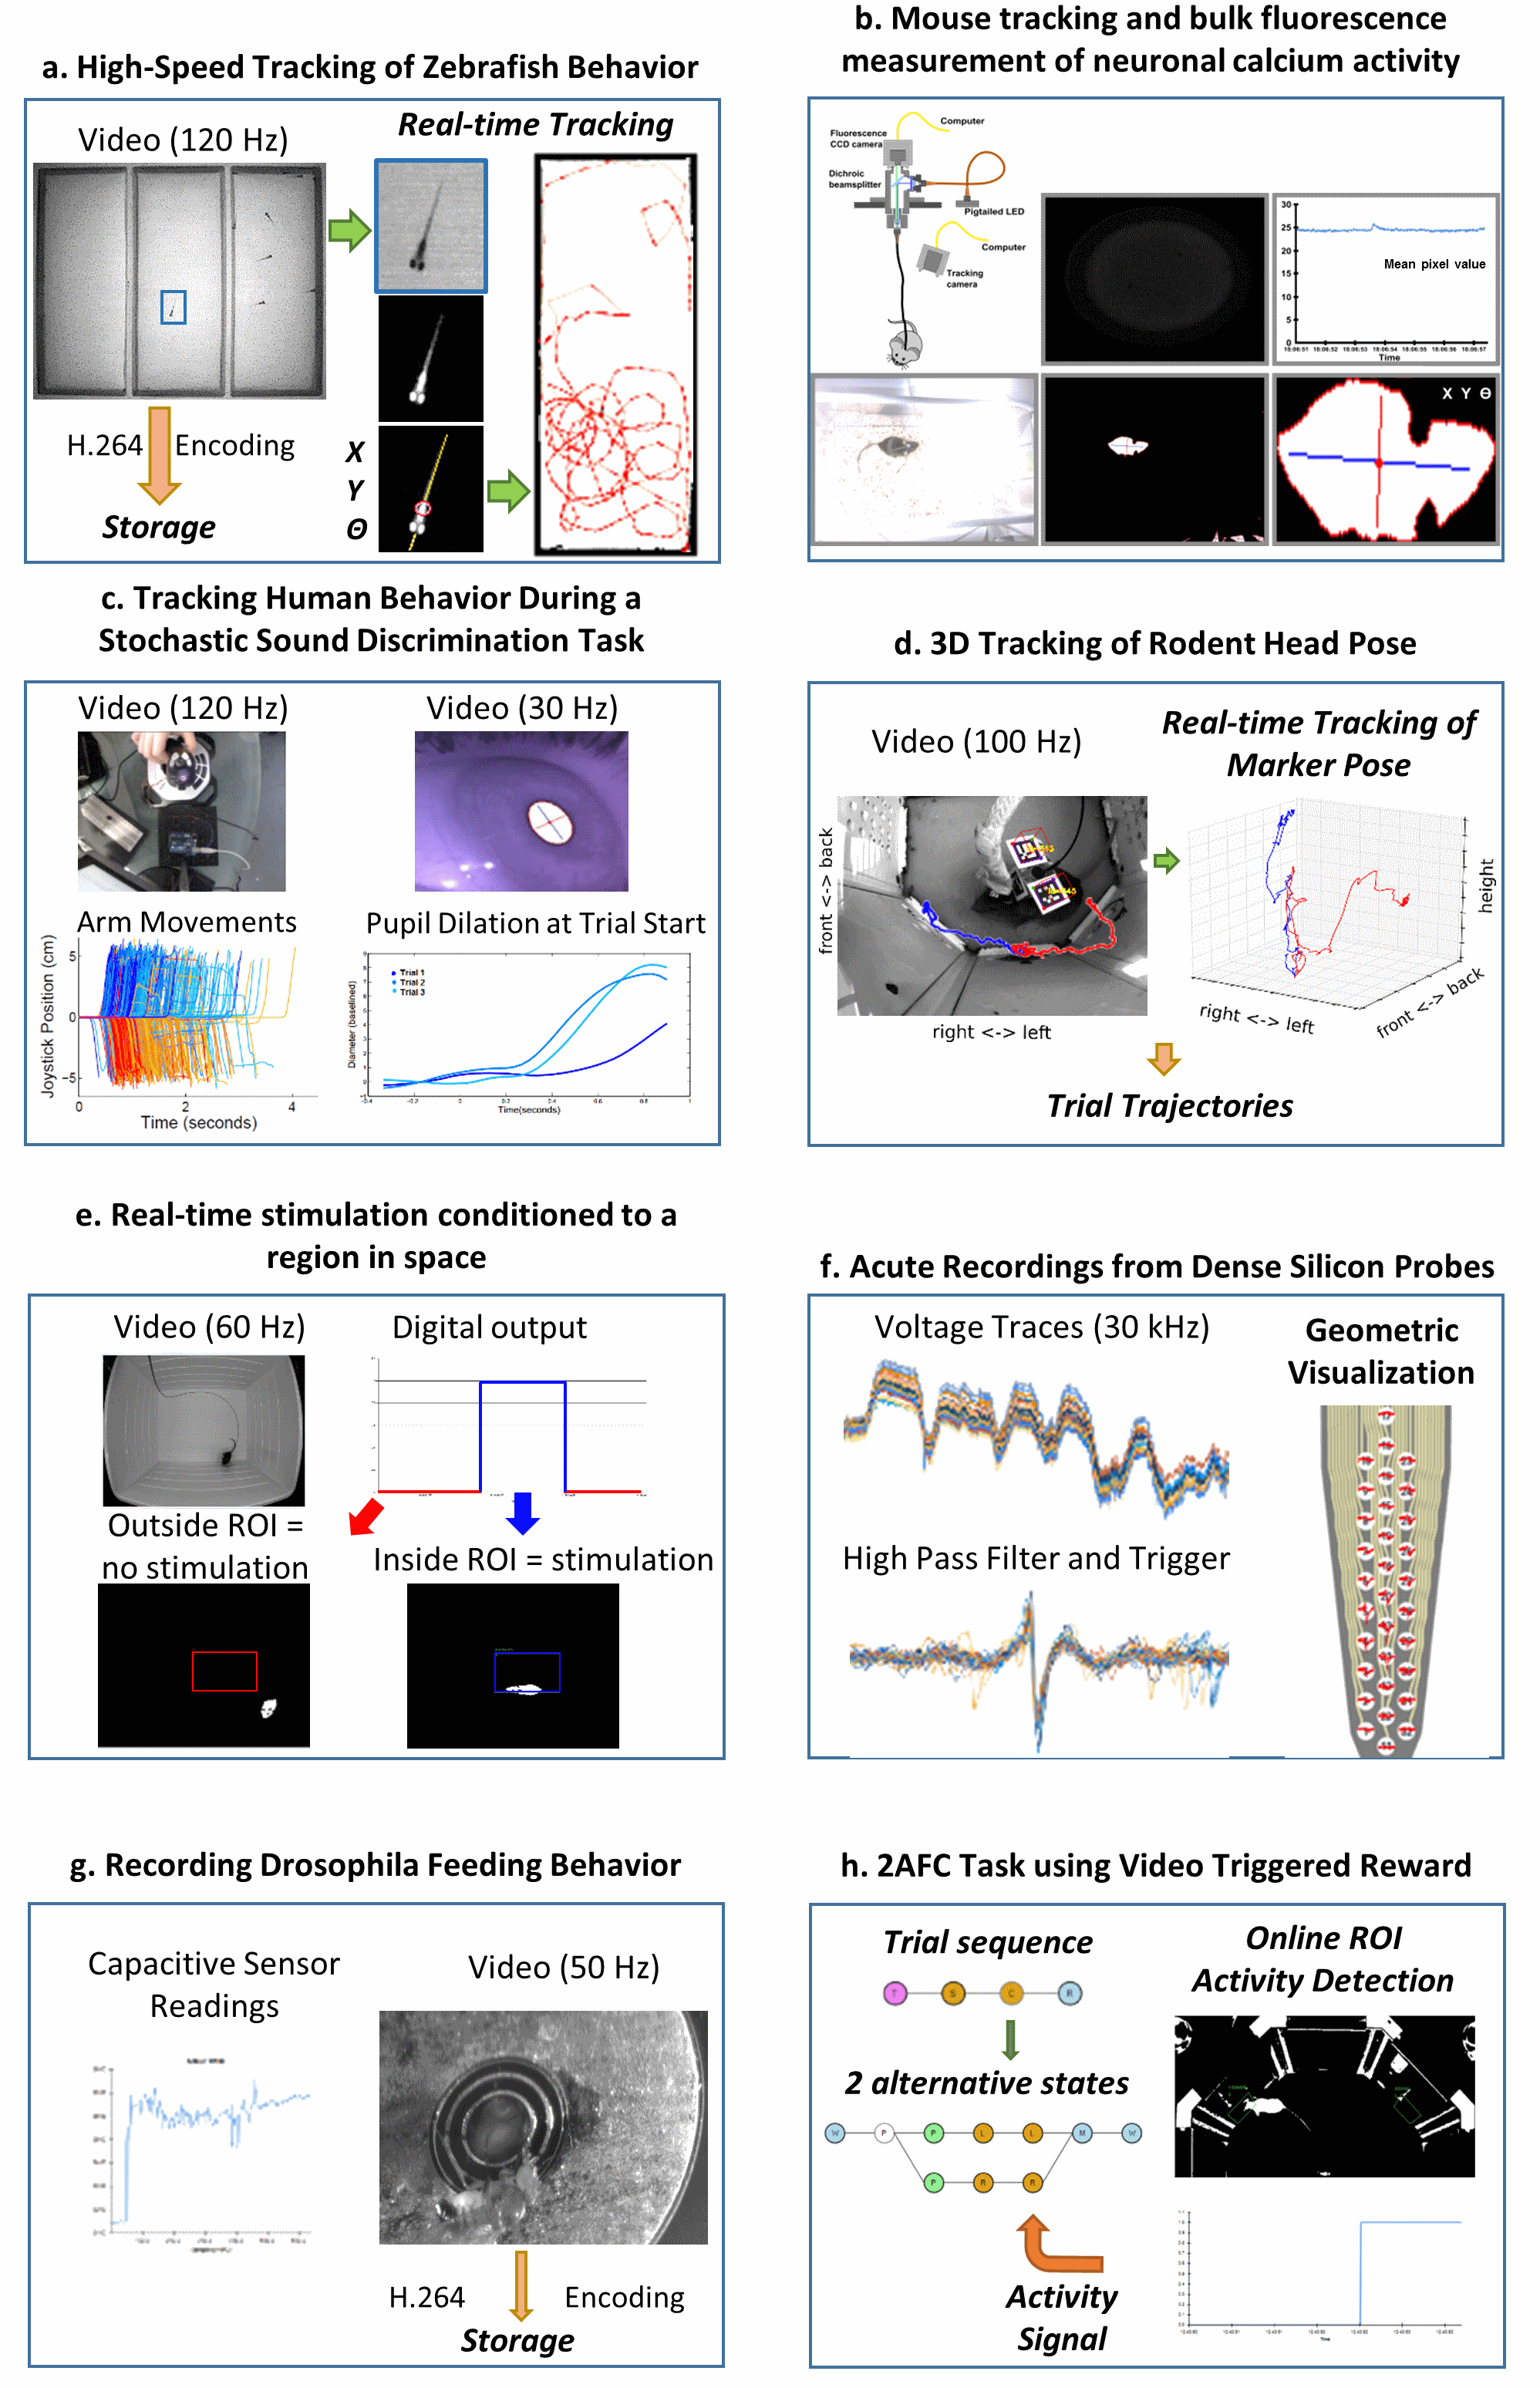
\includegraphics[width=\linewidth]{chapters/figuresChTools/bonsaiApplications.png}}
\end{center}
\vspace{-5mm}
\caption{Example neuroscience experimental setups using Bonsai.}
\label{fig:bonsaiApplications}
\end{figure}

One of the first use cases driving the development of Bonsai was the automated online tracking of animal behaviour using video. The most common tracking application involves chaining together operators for image segmentation and binary region analysis to allow the extraction of the spatial location of an animal over time (Figures \ref{fig:bonsaiApplications}A,B). The same technique can easily be extended to track different kinds of objects, such as eyes or experimental manipulanda in human psychophysics experiments (Figure \ref{fig:bonsaiApplications}C), provided adequate illumination contrast and the appropriate choice of a method for segmentation. These image processing tools can also be used to acquire and process physiological data in neural imaging setups, where it is now possible to record bioluminescent or fluorescent reporters of neural activity during behaviour. For example, Figure \ref{fig:bonsaiApplications}B demonstrates simultaneous measurement of animal behaviour and neural activity using bulk fluorescence calcium imaging in the mouse brain recorded with a CCD sensor and a fiberoptic system \cite{Tecuapetla2014}.

Raw video data from modern high-resolution, high-speed cameras can be expensive and cumbersome to store. Online video compression and storage sinks were implemented taking advantage of parallelism to avoid frame loss. Video compression is processing intensive and can compromise data acquisition if reading the next frame has to wait for the previous frame to be fully encoded. One solution is to buffer incoming frames and compress them in parallel with the rest of the processing stream. By encapsulating this behaviour into a Bonsai sink, it became easy to incorporate video recording and compression functionality into any image processing pipeline (Figures \ref{fig:bonsaiApplications}A–E,G,H).

While simple image processing techniques can easily extract continuous two-dimensional measures of animal location over time, it often becomes the case that the experimenter is concerned with tracking the detailed behaviour of specific features in the animal's body, such as head pose. This is an essential component in neurophysiology or stimulation experiments in freely moving animals, where ongoing behaviour is the central constraint in interpreting neural responses and manipulations. However, identifying such features and reconstructing their position and orientation in 3D space is a challenging computer vision problem. A common solution is to use planar fiducial markers of known geometry \cite{Kato1999, Garrido-Jurado2014} (Figure \ref{fig:bonsaiApplications}D). The computer vision research community has developed some open-source software solutions to this problem \cite{Garrido-Jurado2014}, which have been integrated into Bonsai to allow the possibility of easily and flexibly incorporating online 3D fiducial tracking in video streams. This approach has been used successfully to record 3D head movements of a mouse under optogenetic stimulation in a decision-making task (Figure \ref{fig:bonsaiApplications}D).

One final, but important application of video stream processing is in the development of closed-loop interfaces, where the actions of an animal directly modulate manipulations under the experimenter's control. This kind of experiment requires fast online analysis of behaviour and physiological variables of interest that are subsequently coupled to hardware control interfaces. In Figure \ref{fig:bonsaiApplications}E, real-time stimulation conditioned to a region in space was implemented by analyzing the position of an animal in a square arena. Whenever the animal found itself inside a specified region of interest, a signal was sent to an Arduino controller which was then used to drive optogenetic stimulation of specific neural circuits.

Another key data type that is commonly processed by Bonsai dataflows is buffered time-series data. This type of data usually arises from audio, electrophysiology or other digital acquisition systems where multiple data samples, from one or more channels, are synchronously acquired, buffered and streamed to the computer. These buffers are often represented as data matrices, where rows are channels and columns represent individual data samples through time, or vice-versa. Support for simple band-pass filters, thresholding and triggering allowed us to build flexible spike detection and waveform extraction systems (Figure \ref{fig:bonsaiApplications}F). Using Intan's Rhythm API, we integrated into Bonsai support for a variety of next-generation electrophysiology devices using Intan's digital amplifier technology, such as the Open Ephys acquisition system \cite{Voigts2013} or Intan's evaluation board (RHD2000, Intan Technologies, US). This system was successfully used to acquire and visualize simultaneous recordings from dense silicon probes where spikes from a loose-patch juxtacellular pipette were used as triggers to align and extract waveform data appearing on the multi-channel extracellular probe. Responses from every silicon probe site could then be superimposed on an accurate rendition of the probe geometry, in real-time.

The ability to rapidly integrate new modules allowed us to support the development and cross-validation of new tools for behavioral neuroscience. A paradigmatic example was the flyPAD, a new method for quantifying feeding behaviour in Drosophila melanogaster by measuring changes in electrode capacitance induced by the proboscis extension of a fly \cite{Itskov2014}. The integration of the flyPAD in Bonsai allowed researchers to quickly get started using this approach to design new experiments. Furthermore, it also allowed the validation of the tool by enabling simultaneous acquisition of high-speed video recordings of fly behaviour which were later used for annotation and classification of the sensor feeding traces (Figure \ref{fig:bonsaiApplications}G).

In a different set of experiments, Bonsai was used to implement a variation on a popular two-alternative forced choice (2AFC) decision-making task for rodents (Figure \ref{fig:bonsaiApplications}H). In this type of task, animals are placed in an environment with three “ports.” They are presented with a stimulus in the center port and afterwards report their perception of the stimulus by going either to the left or right choice ports. In the variation we present in this work, the two choice ports were replaced by regions of interest where the activity of the animal is analyzed using computer vision. This example offered unique challenges as it combined sophisticated sequential control of a task environment with continuous data stream processing of video and sensor data.

The integration of all these diverse components for data acquisition and experiment control does not only allow for the rapid deployment of established protocols. In fact, the modular nature of their integration (i.e., how they can be combined together) opens up new avenues for research, by allowing a rich, rapid exploration of novel methodologies. To demonstrate this, we created a dynamic virtual environment for freely moving rodents where the visual presentation of a stimulus is tightly controlled in closed-loop to the actions of the animal. We used a projection setup similar to the low-cost multi-touch sensing table proposed by \cite{Han2005}, where a visible light rear-projection system is coupled with infrared illumination and an infrared imaging sensor to detect in real-time where the animal is located with respect to the visual display surface (Supplementary Video 2).

\subsection{Discussion}

After about a year of using Bonsai in an active neuroscience research institute, dozens of different experimental protocols and data analysis pipelines have been successfully implemented using the provided building blocks \cite{Gouvea2014, Itskov2014, Tecuapetla2014}. We were surprised by the diversity of applications and by the pace at which new modules and devices were developed and integrated.

The performance achieved by Bonsai dataflow processing was an important consideration throughout (Box 2). Video processing can be particularly challenging to handle given the bandwidth required to quickly acquire and process large data matrices. In order to correlate continuous measures of behaviour with neural activity, it is useful for those measurements to have both high spatial and high temporal resolution. Using Bonsai, we were able to simultaneously process and compress grayscale image sequences from high resolution ($1280 \times 960$) and high frame rate (120 Hz) cameras using standard off-the-shelf desktop computers (Intel Core i7, 8 GB RAM). In fact, many of the reported assays use multiple (>2) such video streams with success and actually process the behaviour video online either to control states of the behaviour protocol or to pre-process video data for offline analysis.

One of the areas where we see the application of Bonsai becoming most significant is in the development of dynamic behaviour assays (environments) using reactive control strategies. Brains evolved to generate and control behaviors that can deal with the complexity of the natural world. However, when neuroscientists try to investigate these behaviors in the lab, it is often difficult to design equivalent environmental complexity in a controlled manner. As an example, consider a simple foraging scenario in which a land animal must collect, in a timely manner, food items that become available at random intervals in many sites. If the item is not collected in time, it rots or gets eaten by competitors. In the case of a single foraging site, a FSM description intuitively represents the workings of the environment (Figure \ref{fig:bonsaiStateMachine}A). However, let us now consider a situation where the environment has two of these food sites operating independently, thus introducing the possibility of different events occurring simultaneously at each of the sites. If our environment is modeled as a finite-state machine, then we must represent every possible combination of states and transitions, as in Figure \ref{fig:bonsaiStateMachine}B. In the classical state machine formalism the machine can only be in one state at a time, which means we now need to model each state as the combination of the individual independent states at each reward location. Furthermore, because transitions between these states are asynchronous and independent, we thus have edges between nearly every pair of nodes, as each reward site can change its state at any point in time relative to the other.

\begin{figure}
\begin{center}
\scalebox{1.00}{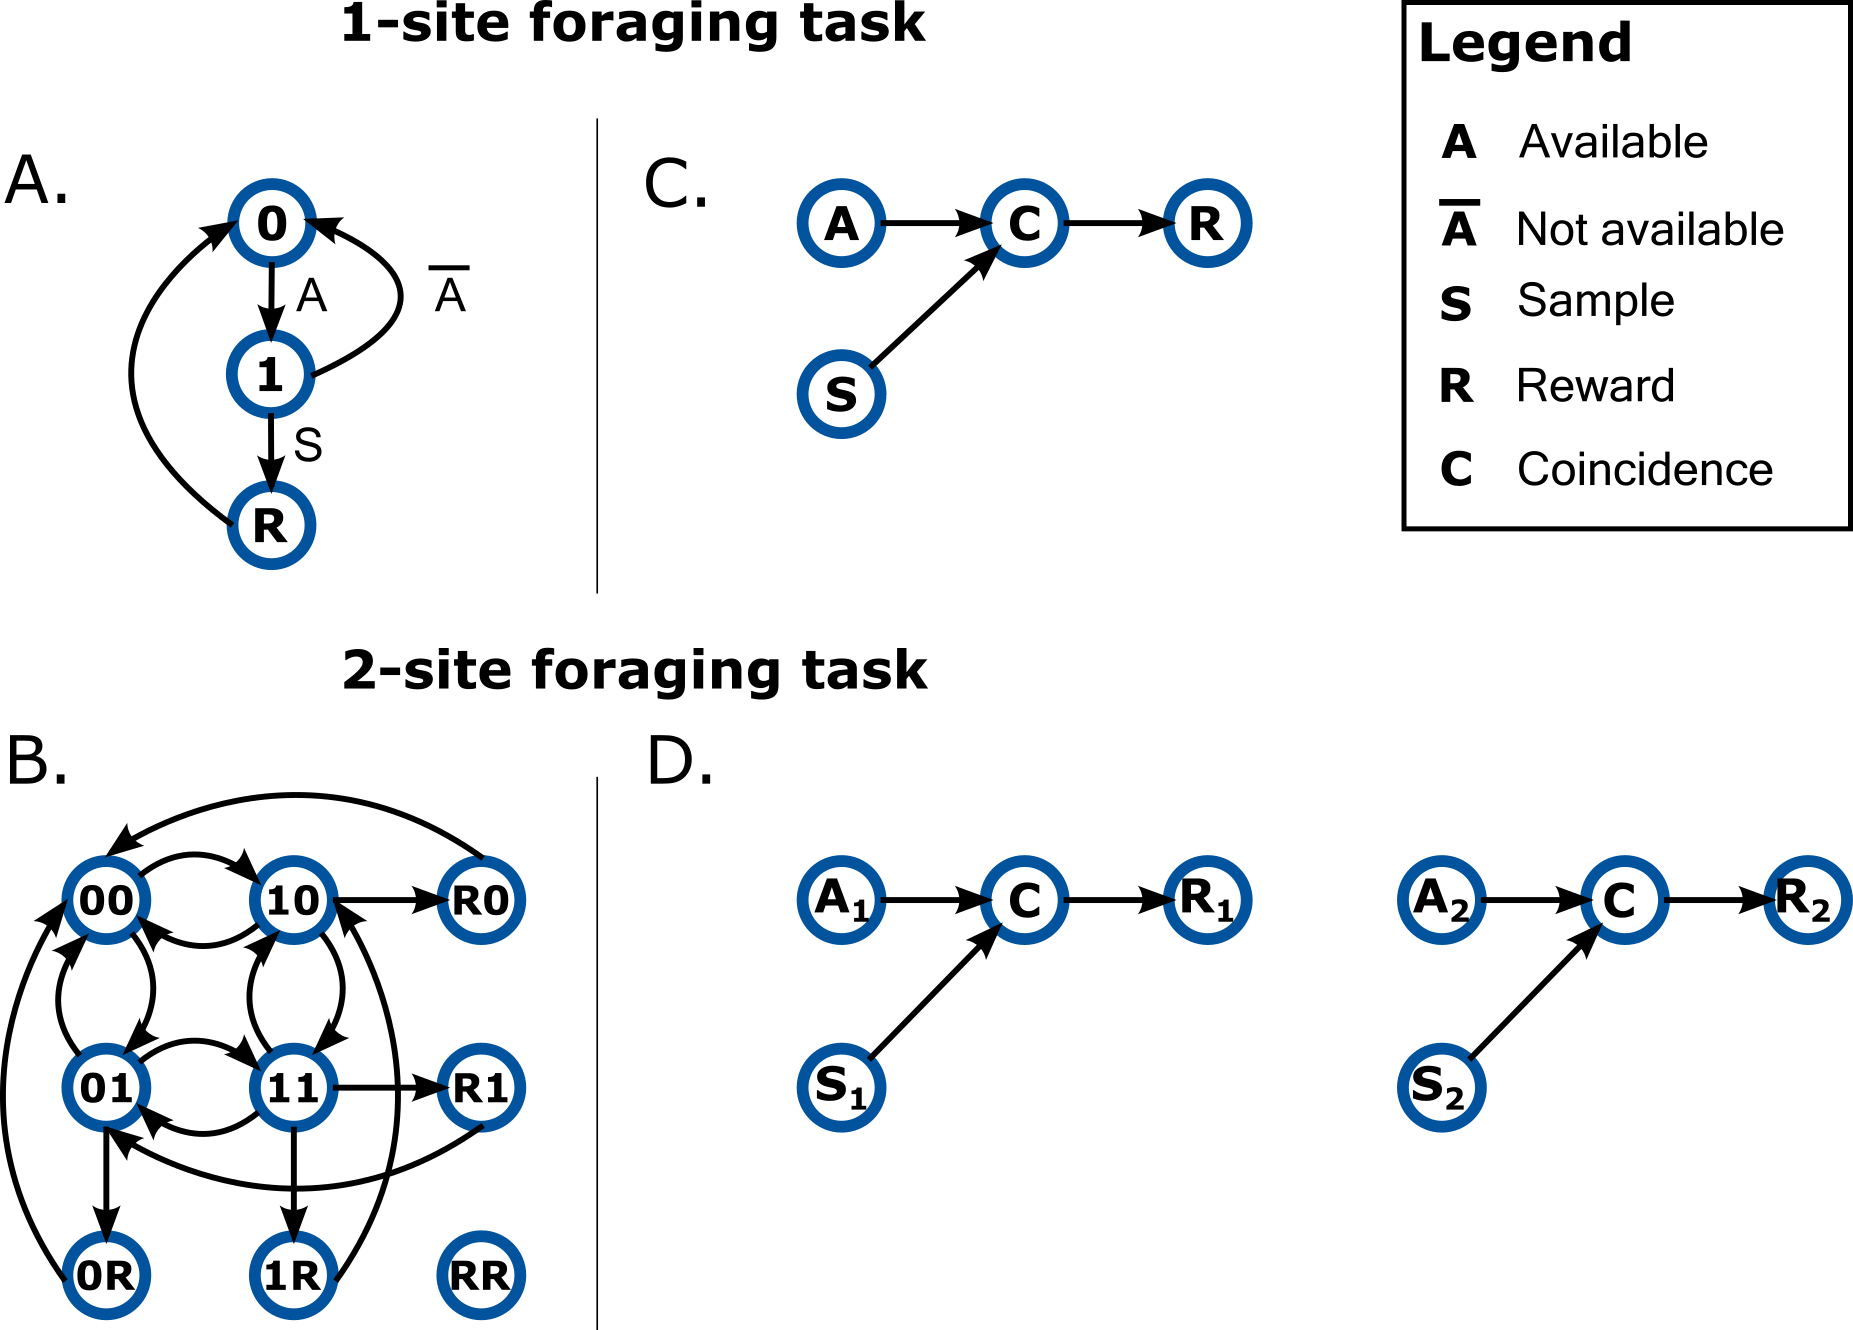
\includegraphics[width=\linewidth]{chapters/figuresChTools/bonsaiStateMachine}}
\end{center}
\vspace{-5mm}
\caption{Describing the behaviour of dynamic environments using either state-machines or dataflows.}
\label{fig:bonsaiStateMachine}
\end{figure}

How would designing such a scenario feel like in a reactive programming language? Figure \ref{fig:bonsaiStateMachine}C shows a possible specification of the 1-site foraging task in reactive terms. In this case, we have two sources of events from the environment: one timer signaling the availability of reward (A); and a sampling event (S) which is triggered every time the animal checks the location for food. Both of these events can occur independently of each other, but when a sampling event coincides with reward availability (C), then reward (R) is delivered. Because this description is intrinsically asynchronous and parallel, it makes it extremely easy to scale the task to a larger set of locations: just replicate the dataflow for each of the other locations (Figure \ref{fig:bonsaiStateMachine}D). In this example, the design space was made more intuitive by introducing the parallel and asynchronous nature of a real-world situation into our modeling formalism.

Another difficulty of the classical state machine formalism is dealing with continuous variables. The natural environment provides constant real-time feedback that tightly correlates with the actions of an animal. Reproducing such closed-loop interaction and manipulating its dynamics is a necessary tool for fully investigating brain function. Such models are virtually impossible to represent in a machine of finite states, given the potential infinitude of feedback responses. However, the dataflow formalism of asynchronous event sources can easily accommodate such models. In fact, this is their natural battleground; nodes represent reactive operators that promptly respond to input values broadcasted by event sources. These models of asynchronous computation are thus ideal for recreating the complex discrete and continuous aspects of natural environments that brains evolved to master. We thus propose Bonsai as a new tool for neuroscientists trying to understand how the brain deals with real world complexity.

\pagebreak







\chapter{Moving with and without Motor Cortex}
\epigraph{I first became sceptical of the supposed path of the conditioned reflex when I found that rats, trained in a differential reaction to light, showed no reduction in accuracy of performance when almost the entire motor cortex, along with the frontal poles of the brain, was removed.}{\textsc{Karl S. Lashley}, \textit{In Search of the Engram} (1950)}
				
% !TEX root = ../ThesisTemplateCNP.tex
	
	
% Chapter summary
				
\section{Chapter Summary}

The role of motor cortex in the direct control of movement remains unclear, particularly in non-primate mammals. More than a century of research using stimulation, anatomical and electrophysiological studies has implicated neural activity in this region with all kinds of movement. However, following the removal of motor cortex, or even the entire cortex, rats retain the ability to execute a surprisingly large range of adaptive behaviours, including previously learned skilled movements. In this chapter we revisit these two conflicting views of motor cortical control by asking what the primordial role of motor cortex is in non-primate mammals, and how it can be effectively assayed. In order to motivate the discussion we present a new assay of behaviour in the rat, challenging animals to produce robust responses to unexpected and unpredictable situations while navigating a dynamic obstacle course. Surprisingly, we found that rats with motor cortical lesions show clear impairments in dealing with an unexpected collapse of the obstacles, while showing virtually no impairment with repeated trials in many other motor and cognitive metrics of performance. Finally, we present the results of a preliminary investigation on the neurobiological basis of robust responses using electrocorticography and report the existence of large amplitude evoked potentials in the rat motor cortex following exposure to occasionally unstable obstacles.

\pagebreak




% Videos

\videolabel{vid:learning}
\videolabel{vid:learning-matrix}
\videolabel{vid:decorticate-habituation}

\videolabel{vid:conditions}
\videolabel{vid:jpak20}

\videolabel{vid:manipulation-strategies}
\videolabel{vid:manipulation-small}
\videolabel{vid:manipulation-large}

\videolabel{vid:manipulation-decorticate-oblivious}
\videolabel{vid:manipulation-decorticate-halting}


% Introduction
\section{Introduction}

Since its discovery 150 years ago, the role of motor cortex has been a topic of controversy and confusion \cite{Tyler2000,Gross2007,Lashley1924,DeBarenne1933}. Here we report our efforts to establish a teleology for cortical motor control. Motor cortex may play roles in ``understanding'' the movements of others \cite{Rizzolatti2004}, imagining one's own movements \cite{Porro1996}, or in learning new movements \cite{Kawai2015}, but here we will focus on its role in directly controlling movement.

\subsubsection*{Stimulating motor cortex causes movement; motor cortex is active during movement}

Motor cortex is broadly defined as the region of the cerebral hemispheres from which movements can be evoked by low-current stimulation, following Fritsch and Hitzig's original experiments in 1870 \cite{Fritsch1870}. Stimulating different parts of the motor cortex elicits movement in different parts of the body, and systematic stimulation surveys have revealed a topographical representation of the entire skeletal musculature across the cortical surface \cite{Leyton1917, Penfield1937, Neafsey1986}. Electrophysiological recordings in motor cortex have routinely found correlations between neural activity and many different movement parameters, such as muscle force \cite{Evarts1968}, movement direction \cite{Georgopoulos1986}, speed \cite{Schwartz1993}, or even anisotropic limb mechanics \cite{Scott2001} at the level of both single neurons \cite{Evarts1968,Churchland2007} and populations \cite{Georgopoulos1986,Churchland2012}. Determining what exactly this activity in motor cortex controls \cite{Todorov2000} has been further complicated by studies using long stimulation durations in which continuous stimulation at a single location in motor cortex evokes complex, multi-muscle movements \cite{Graziano2002,Aflalo2006}. However, as a whole, these observations all support the long standing view that activity in motor cortex is involved in the direct control of movement.

\subsubsection*{Motor cortex lesions produce different deficits in different species}

What types of movement require motor cortex? In humans, a motor cortical lesion is devastating, resulting in the loss of muscle control or even paralysis; movement is permanently and obviously impaired \cite{Laplane1977}. In non-human primates, similar gross movement deficits are observed after lesions, albeit transiently \cite{Leyton1917}. The longest lasting effect of a motor cortical lesion is the decreased motility of distal forelimbs, especially in the control of individual finger movements required for precision skills \cite{Leyton1917,Darling2011}. But equally impressive is the extent to which other movements fully recover, including the ability to sit, stand, walk, climb and even reach to grasp, as long as precise finger movements are not required \cite{Leyton1917,Darling2011,Zaaimi2012}. In non-primate mammals, the absence of lasting deficits following motor cortical lesion is even more striking. Careful studies of skilled reaching in rats have revealed an impairment in paw grasping behaviours \cite{Whishaw1991,Alaverdashvili2008a}, comparable to the long lasting deficits seen in primates, but this is a limited impairment when compared to the range of movements that \emph{are} preserved \cite{Whishaw1991,Kawai2015}. In fact, even after complete decortication, rats, cats and dogs retain a shocking amount of their movement repertoire \cite{Goltz1888,Bjursten1976,Terry1989}. If we are to accept the simple hypothesis that motor cortex is the structure responsible for ``voluntary movement production'', then why is there such a blatant difference in the severity of deficits caused by motor cortical lesions in humans versus other mammals? With over a century of stimulation and electrophysiology studies clearly suggesting that motor cortex is involved in many types of movement, in all mammalian species, how can these divergent results be reconciled?

\subsubsection*{There are anatomical differences in corticospinal projections between primates and other mammals}

In primates, the conspicuous effects of motor cortical lesion can also be produced by sectioning the pyramidal tract, the direct monosynaptic projection that connects motor cortex, and other cortical regions, to the spinal cord \cite{Tower1940,Lawrence1968}. The corticospinal tract is thought to support the low-current movement responses evoked by electrical stimulation in the cortex, as evidenced by the increased difficulty in obtaining a stimulation response following section at the level of the medulla \cite{Woolsey1972}. In monkeys, and similarly in humans, this fibre system has been found to directly terminate on spinal motor neurons responsible for the control of distal muscles \cite{Leyton1917,Bernhard1954}. However, in all other mammals, including cats and rats, the termination pattern of the pyramidal tract in the spinal cord largely avoids these ventral motor neuron pools and concentrates instead on intermediate zone interneurons and dorsal sensory neurons \cite{Kuypers1981,Yang2003}. Furthermore, in humans, the rubrospinal tract---a descending pathway originating in the brainstem and terminating in the intermediate zone---is degenerated compared to other primates and mammals \cite{Square1982}, and is thought to play a role in compensating for the loss of the pyramidal tract in non-human species \cite{Lawrence1968a,Zaaimi2012}. These differences in anatomy might explain the lack of conspicuous, lasting movement deficits in non-primates, but leaves behind a significant question: what is the motor cortex actually controlling in all these other mammals?

\subsubsection*{What is the role of motor cortex in non-primate mammals?}

In the rat, a large portion of cortex is considered ``motor'' based on anatomical \cite{Donoghue1982}, stimulation \cite{Donoghue1982,Neafsey1986} and electrophysiological evidence \cite{Hyland1998}. However, the most consistently observed long-term deficit following motor cortical lesion has been an impairment in supination of the wrist and individuation of digits during grasping, which in turn impairs reaching for food pellets through a narrow vertical slit \cite{Whishaw1991,Alaverdashvili2008a}. Despite the fact that activity in rodent motor cortex has been correlated with movements in every part of the body (not just distal limbs) \cite{Hill2011,Erlich2011}, it would appear we are led to conclude that this large high-level motor structure, with dense efferent projections to motor areas in the spinal cord \cite{Kuypers1981}, basal ganglia \cite{Turner2000,Wu2009}, thalamus \cite{Lee2008}, cerebellum \cite{Baker2001} and brainstem \cite{Jarratt1999}, as well as to most primary sensory areas \cite{Petreanu2012,Schneider2014}, evolved simply to facilitate more precise wrist rotations and grasping gestures. Maybe we are missing something. Might there be other problems in movement control that motor cortex is solving, but that we may be overlooking with our current assays?

\subsubsection*{A role in modulating the movements generated by lower motor centres}

A different perspective on motor cortex emerged from studying the neural control of locomotion, suggesting that the corticospinal tract plays a role in the \emph{adjustment} of ongoing movements that are generated by lower motor systems. In this view, rather than motor cortex assuming direct control over muscle movement, it instead modulates the activity and sensory feedback in spinal circuits in order to adapt a lower movement controller to challenging conditions. This idea that the descending cortical pathways superimpose speed and precision on an existing baseline of behaviour was also suggested by lesion work in primates \cite{Lawrence1968a}, but has been investigated most thoroughly in the context of cat locomotion.

It has been known for more than a century that completely decerebrate cats are capable of sustaining the locomotor rhythms necessary for walking on a flat treadmill utilizing only spinal circuits \cite{GrahamBrown1911}. Brainstem and midbrain circuits are sufficient to initiate the activity of these spinal central pattern generators \cite{Grillner1973}, so what exactly is the contribution of motor cortex to the control of locomotion? Single-unit recordings of pyramidal tract neurons (PTNs) from cats walking on a treadmill have shown that a large proportion of these neurons are locked to the step cycle \cite{Armstrong1984a}. However, we know from the decerebrate studies that this activity is not necessary for the basic locomotor pattern. What then is its role?

Lesions of the lateral descending pathways (containing corticospinal and rubrospinal projections) produce a long term impairment in the ability of cats to step over obstacles \cite{Drew2002}. Recordings of PTN neurons during locomotion show increased activity during these visually guided modifications to the basic step cycle \cite{Drew1996}. These observations suggest that motor cortex neurons are necessary for precise stepping and adjustment of ongoing locomotion to changing conditions. However, long-term effects seem to require complete lesion of \emph{both} the corticospinal and rubrospinal tracts \cite{Drew2002}. Even in these animals, the voluntary act of stepping over an obstacle does not disappear entirely, and moreover, they can adapt to changes in the height of the obstacles \cite{Drew2002}. Specifically, even though these animals never regain the ability to gracefully clear an obstacle, when faced with a higher obstacle, they are able to adjust their stepping height in such a way that would have allowed them to comfortably clear the lower obstacle \cite{Drew2002}. Furthermore, deficits caused by lesions restricted to the pyramidal tract seem to disappear over time \cite{Liddell1944}, and are most clearly visible only the first time an animal encounters a new obstacle \cite{Liddell1944}.

The view that motor cortex in non-primate mammals is principally responsible for adjusting ongoing movement patterns generated by lower brain structures is appealing. What is this modulation good for? What does it allow an animal to achieve? How can we assay its necessity?

\subsubsection*{Towards a new teleology; new experiments required}

It should now be clear that the involvement of motor cortex in the direct control of all ``voluntary movement'' is human-specific. There is a role for motor cortex across mammals in the control of precise movements of the extremities, especially those requiring individual movements of the fingers, but these effects are subtle in non-primate mammals. Furthermore, what would be a devastating impairment for humans may not be so severe for mammals that do not depend on precision finger movements for survival. Therefore, generalizing this specific role of motor cortex from humans to all other mammals would be misleading. We could be missing another, more primordial role for this structure that predominates in other mammals, and by doing so, we may also be missing an important role in humans.

The proposal that motor cortex induces modifications of ongoing movement synergies, prompted by the electrophysiological studies of cat locomotion, definitely points to a role consistent with the results of various lesion studies. However, in assays used, the ability to modify ongoing movement generally recovers after a motor cortical lesion. What are the environmental siutations in which motor cortical modulation is most useful?

Cortex has long been proposed to be the structure responsible for integrating a representation of the world and improving the predictive power of this representation with experience \cite{Barlow1985,Doya1999}. If motor cortex is the means by which these representations can gain influence over the body, however subtle and ``modulatory'', can we find situations (i.e. tasks) in which this cortical control is required?

The necessity of cortex for various behavioural tasks has been actively investigated in experimental psychology for over a century, including the foundational work of Karl Lashley and his students \cite{Lashley1921a,Lashley1950a}. In the rat, large cortical lesions were found to produce little to no impairment in movement control, and even deficits in learning and decision making abilities were difficult to demonstrate consistently over repeated trials. However, Lashley did notice some evidence that cortical control may be involved in postural adaptations to unexpected perturbations \cite{Lashley1921a}. These studies once again seem to recapitulate the two most consistent observations found across the entire motor cortical lesion literature in non-primate mammals since Hitzig \cite{Fritsch1870}, Goltz \cite{Goltz1888}, Sherrington \cite{Sherrington1885} and others \cite{Oakley1979,Terry1989}. One, direct voluntary control over movement is most definitely not abolished through lesion; and two, certain aspects of some movements are definitely impaired, but only under certain challenging situations. The latter are often reported only anecdotally. It was this collection of intriguing observations in animals with motor cortical lesions that prompted us to expand the scope of standard laboratory tasks to include a broader range of motor control challenges that brains encounter in their natural environments.

In the following, we report an experiment that was designed to provide controlled exposure of animals to more naturally challenging environments. The results of this experiment have led us to formulate a new teleology for cortical motor control that we will present in the discussion.

\section{Experiment Introduction}

In the natural world, an animal must be able to adapt locomotion to any surface, not only in anticipation of upcoming terrain, but also in response to the unexpected perturbations that often occur during movement. This allows animals to move robustly through the world, even when navigating a changing environment. Testing the ability of the motor system to generate a robust response to an unexpected change can be difficult as it requires introducing a perturbation without cueing the animal about the altered state of the world. Marple-Horvat and colleagues built a circular ladder assay for cats that was specifically designed to record from motor cortex during such conditions \cite{Marple-Horvat1993}. One of the modifications they introduced was to make one of the rungs of the ladder fall unexpectedly under the weight of the animal. When they recorded from motor cortical neurons during the rung drop, they noticed a marked increase in activity, well above the recorded baseline from normal stepping, as the animal recovered from the fall and resumed walking. However, whether this increased activity of motor cortex was necessary for the recovery response has never been assayed.


% Methods
\section{Methods}

\textbf{Lesions:} Ibotenic acid was injected bilaterally in 7 Long-Evans rats (ages from 83 to 141 days; 5 females, 2 males), on 3 injection sites at 2 depths (\SI{-1.5}{\milli\meter} and \SI{-0.75}{\milli\meter} from the surface of the brain). At each depth we injected a total amount of \SI{82.8}{\nano\liter} using a microinjector (Drummond Nanoject II, \SI{9.2}{\nano\liter} per injection, 9 injections per depth). The coordinates for each site, in \si{\milli\meter} with respect to Bregma, were: +1.0 AP / 2.0 ML; +1.0 AP / 4.0 ML; +3.0 AP / 2.0 ML. Five other animals were used as sham controls (age-matched controls; 3 females, 2 males), subject to the same intervention, but where ibotenic acid was replaced with physiological saline. Two additional animals were left as wildtype controls (age-matched controls; 2 females).

\textbf{Recovery period:} After the surgeries, animals were given a minimum of one week (up to two weeks) recovery period in isolation. After this period, animals were handled every day for a week, after which they were paired again with their age-matched control to allow for social interaction during the remainder of the recovery period. In total, all animals were allowed at least one full month of recovery before they were first exposed to the behaviour assay.

\textbf{Histology:} Animals were perfused intracardially with 4\% paraformaldehyde in phosphate buffer saline (PBS) and brains were post-fixed for at least \SI{24}{\hour} in the same fixative. Serial coronal sections (\SI{100}{\micro\meter}) were Nissl-stained and imaged for identification of lesion boundaries.

\textbf{Behaviour:} The animals were kept in a state of water deprivation for \SI{20}{\hour} before each daily session. During the session the animal was placed inside a behaviour box for \SI{30}{\minute}, where it could collect water by shuttling back and forth between two reward ports (Island Motion Corporation, USA). To do this, animals had to cross a \SI{48}{\centi\meter} obstacle course composed of eight \SI{2}{\centi\meter} aluminum steps spaced by \SI{4}{\centi\meter}. The structure of the behaviour assay and each step in the obstacle course was built out of Bosch Rexroth aluminum structural framing, \SI{20}{\milli\meter} series. For every trial, rats were delivered a \SI{20}{\micro\liter} drop of water. At the end of the day, rats were given free access to water for \SI{10}{\minute} before initiating the next deprivation period.

A motorized brake allowed us to lock or release each step in the obstacle course using an Arduino and custom control software. The shaft of each of the obstacles was coupled to an acrylic piece used to control the rotational stability of each step. In order to lock a step in a fixed position, two servo motors are actuated to press against the acrylic piece and hold it in place. Two other acrylic pieces are used as stops to ensure a maximum rotation angle of approximately +/- \ang{100}. Two small nuts were attached to the bottom of each step to work as light weights that give the obstacles a tendency to return to their original flat configuration. In order to ensure that noise from servo motor actuation cannot be used as a cue to tell the animal about the state of each step, the motors are always set to press against an acrylic piece, either the piece that keeps the step stabilized, or the acrylic stops. At the beginning of each trial, the motors go through a randomized sequence of positions in order to mask information about state transitions and also to ensure the steps are reset to their original configuration.

Animals were run on \SI{30}{\minute} sessions every day of the week from Monday to Saturday, with a day of free access to water on Sunday. Before the water deprivation begins, animals were run on a single habituation session where they were placed in the box for a period of \SI{15}{\minute}. Animals were run on the following sequence of conditions over the course of a month: day 0, habituation to the box; day 1-4, all the steps were fixed in a stable configuration; day 5, 20 trials of the stable configuration, after which the two center steps are made free to rotate; day 6-10, the center two steps remain free to rotate; day 11, 20 trials of the partially unstable configuration, after which the two center steps are again fixed in a stable state; day 12, all the steps were fixed in a stable configuration; day 13-16, the state of the center two steps was randomized on a trial-by-trial basis to be either stable or free to rotate; day 17-18, 20 trials of stable configuration, followed by the randomized protocol for the center two steps; day 19-22, the state of the six center steps was randomized trial-by-trial in such a way that on each trial either two rails are picked at random to be free to rotate or with a low probability all rails are stable; day 23, after 20 trials of randomized permutations, all rails are made free to rotate; day 24, all rails are free to rotate.

\textbf{Behaviour Data:} The performance of the animals was recorded using a high-speed and high-resolution video camera (PointGrey Flea3 FL3-U3-13S2M-CS, 1280x960 @ 120 fps). Behaviour was run in the dark, under infrared illumination using super-bright LED strips. Tracking of the nose was achieved by background subtraction and connected component labeling of segmented image elements, of which we then selected the furthermost point along the major axis of the ellipse best fit to the largest segmented object.

\textbf{Video Classification:} Ethogram classification was done on a frame-by-frame analysis of the high-speed video aligned on first contact with the manipulated rail. The frame of first contact was defined as the first frame in which there is noticeable movement of the rail caused by animal contact. Three main categories of behaviour were observed to follow the first contact: compensation, investigation and halting. Behaviour sequences were first classified as belonging to one of these categories and their onsets and offsets determined by the following criteria. Compensation behaviour is defined by rapid, whole-body movement that results in an adaptive postural correction to the perturbation. Onset of this behaviour is defined by the first frame in which there is visible rapid contraction of the body musculature following first contact. Investigation behaviour consists of periods of targeted interaction with the rails, often involving manipulation of the freely moving obstacle with the forepaw. The onset of this behaviour is defined by the animal orienting its head down to one of the manipulated rails, followed by subsequent interaction. Halting behaviour is characterized by a period in which the animals stop their ongoing motor program, and maintain the same body posture for several seconds, with occasional movements of the head, but without orienting specifically to the manipulated rails. They tend to look up and to the sides as if in a state of confusion, or uncertainty about what to do next. Onset of this behaviour is defined by the moment where locomotion and other motor activities besides movement of the head come to a stop. A human classifier blind to the lesion condition was given descriptions of each of these three main categories of behaviour and asked to note onsets and offsets of each behaviour throughout the video.

\textbf{Data Analysis:} Analysis was run using the NumPy scientific computing package for the Python programming language and custom software.













% Results
\section{Results}

To investigate whether the intact motor cortex is required for the robust control of movement in response to unexpected perturbations, we designed a reconfigurable dynamic obstacle course where individual steps can be made stable or unstable on a trial-by-trial basis (Figure \ref{fig:assay}, also see Methods). In this assay, rats shuttle back and forth across the obstacles, in the dark, in order to collect water rewards. We specifically designed the assay such that modifications to the physics of the obstacles could be made covertly. In this way, the animal has no explicit information about the state of the steps until it actually contacts them. Water deprived animals were trained daily for 4 weeks, throughout which they encountered increasingly challenging states of the obstacle course. Our goal was to characterize precisely the conditions under which motor cortex becomes necessary for the control of movement, and this motivated us to introduce an environment with graded levels of uncertainty.

We compared the performance of 22 animals: 11 with bilateral ibotenic acid lesions to the primary and secondary forelimb motor cortex, and 11 age and gender matched controls (5 sham surgery, 6 wild-types). Animals were given ample time to recover, 4 weeks post-surgery, in order to specifically isolate behaviours that are chronically impaired in animals lacking the functions enabled by motor cortical structures. Histological examination of serial coronal sections revealed significant variability in the extent of damaged areas (Figure \ref{fig:histology}), which was likely caused by mechanical blockage of the injection pipette during lesion induction at some sites. Nevertheless, volume reconstruction of the serial sections allowed us to accurately quantify the size of each lesion, identify each animal (from Lesion A to Lesion K; largest to smallest), and use these values to compare observed behavioural effects as a function of lesion size.

\begin{figure}
\centering
\includestandalone[scale=0.85]{chapters/figuresChBehaviour/histology}
\caption{Histological analysis of lesion size. (\textbf{A}) Representative example of Nissl-stained coronal section showing bilateral ibotenic acid lesion of primary and secondary forelimb motor cortex. (\textbf{B}) Distribution of lesion volumes in the left and right hemispheres for individual animals. A lesion was considered ``large'' if the total lesion volume was above \SI{15}{\milli\meter\cubed}. (\textbf{C}) Super-imposed reconstruction stacks for all the small lesions ($n = 6$). (\textbf{D}) Super-imposed reconstruction stacks for all the large lesions ($n = 5$).}
\label{fig:histology}
\end{figure}

During the first sessions in the ``stable'' environment, all animals, both lesions and controls, quickly learned to shuttle across the obstacles, achieving stable, skilled performance after a few days of training (Figure \ref{fig:learning}). Even though the distance between steps was fixed for all animals, the time taken to adapt the crossing strategy was similar irrespective of body size. When first encountering the obstacles, animals adopted a cautious gait, investigating the location of the subsequent obstacle with their whiskers, stepping with the leading forepaw followed by a step to the same position with the trailing paw (Video \ref{vid:learning}: ``First Leftwards Crossing''). However, over the course of only a few trials, all animals exhibited a new strategy of ``stepping over'' the planted forepaw to the next obstacle, suggesting an increased confidence in their movement strategy in this novel environment (Video \ref{vid:learning}: ``Second Leftwards Crossing''). This more confident gait developed into a coordinated locomotion sequence after a few additional training sessions (Video \ref{vid:learning}: ``Later Crossing''). The development of the ability to move confidently and quickly over the obstacle course was observed in both lesion and control animals (Video \ref{vid:learning-matrix}).

In addition to the excitotoxic lesions, in three animals we performed larger frontal cortex aspiration lesions in order to determine whether the remaining trunk and hindlimb representations were necessary to navigate the elevated obstacle course. Also, in order to exclude the involvement of other corticospinal projecting regions in the parietal and rostral visual areas \cite{Miller1987}, we included three additional animals which underwent even more extensive cortical lesion procedures (Figure \ref{fig:extended}A,B, see Methods). These \emph{extended} lesion animals were identified following chronological order (from Extended Lesion A to Extended Lesion F; where the first three animals correspond to frontal cortex aspiration lesions and the remaining animals to the more extensive frontoparietal lesions). In these extended cortical lesions, recovery was found to be overall slower than in lesions limited to the motor cortex, and animals required isolation and more extensive care during the recovery period.

Nevertheless, when tested in the shuttling assay, the basic performance of these extended lesion animals was similar to that of controls and animals with excitotoxic motor cortical lesions (Figure \ref{fig:extended}C). Animals with large frontoparietal lesions did exhibit a very noticeable deficit in paw placement throughout the early sessions (Figure \ref{fig:extended}D). Interestingly, detailed analysis of paw placement behaviour revealed that this deficit was almost entirely explained by impaired control of the hindlimbs. Paw slips were much more frequent when stepping with a hindlimb than with a forelimb (Figure \ref{fig:extended}E,F). In addition, when a slip did occur, these animals failed to adjust the affected paw to compensate for the fall (e.g. keeping their digits closed), which significantly impacted their overall posture recovery. These deficits in paw placement are consistent with results from sectioning the entire pyramidal tract in cats \cite{Liddell1944}, and reports in ladder walking following motor cortical lesion in rodents \cite{Metz2002}, but surprisingly we did not observe deficits in paw placement in animals with ibotenic acid lesions limited to forelimb motor cortex (Figure \ref{fig:extended}D). Furthermore, despite this initial impairment, animals with extended lesions were still able to improve their motor control strategy up to the point where they were moving across the obstacles as efficiently as controls and other lesioned animals (Figure \ref{fig:extended}C, Video \ref{vid:learning-matrix}). Indeed, in the largest frontoparietal lesion, which extended all the way to rostral visual cortex, recovery of a stable locomotion pattern was evident over the course of just ten repeated trials (Video \ref{vid:decorticate-habituation}). The ability of this animal to improve its motor control strategy in such a short period of time seems to indicate the presence of motor learning, not simply an increase in confidence with the new environment.

In subsequent training sessions we progressively increased the difficulty of the obstacle course, by making more steps unstable. The goal was to compare the performance of the two groups as a function of difficulty. Surprisingly, both lesion and control animals were able to improve their performance by the end of each training stage even for the most extreme condition where all steps were unstable (Figure \ref{fig:learning}, Video \ref{vid:conditions}). This seems to indicate that the ability of these animals to fine-tune their motor performance in a challenging environment remained intact.

One noticeable exception was the animal with the largest ibotenic acid lesion. This animal, following exposure to the first unstable protocol, was unable to bring itself to cross the obstacle course (Video \ref{vid:jpak20}). Some other control and lesioned animals also experienced a similar form of distress following exposure to the unstable obstacles, but eventually all these animals managed to start crossing over the course of a single session. In order to test whether this was due to some kind of motor disability, we lowered the difficulty of the protocol for this one animal until it was able to cross again. Following a random permutation protocol, where any two single steps were released randomly, this animal was then able to cross a single released obstacle placed in any location of the assay. After this success, it eventually learned to cross the highest difficulty level in the assay in about the same time as all the other animals, suggesting that there was indeed no lasting motor execution or learning deficit, and that the disability must have been due to some other unknown, yet intriguing, (cognitive) factor.

Having established that the overall motor performance of these animals was similar across all conditions, we next asked whether there was any difference in the strategy used by the two groups of animals to cross the unstable obstacles. We noticed that during the first week of training, the posture of the animals when stepping on the obstacles changed significantly over time (Figure \ref{fig:posture}B,C). Specifically, the centre of gravity of the body was shifted further forward and higher during later sessions, in a manner proportional to performance. However, after the obstacles changed to the unstable state, we observed an immediate and persistent adjustment of this crossing posture, with animals assuming a lower centre of gravity and reducing their speed as they approached the unstable obstacles (Figure \ref{fig:posture}C,D). Interestingly, we also noticed that a group of animals adopted a different strategy. Instead of lowering their centre of gravity, they either kept it unchanged or shifted it even more forward and performed a jump over the unstable obstacles (Figure \ref{fig:jumping}A,B). These two strategies were remarkably consistent across the two groups, but there was no correlation between the strategy used and the degree of motor cortical lesion (Figure \ref{fig:posture}E,F, \ref{fig:jumping}C). In fact, we found that the use of a jumping strategy was best predicted by the body weight of the animal (Figure \ref{fig:jumping}C).

During the two days where the stable state of the environment was reinstated, the posture of the animals was gradually restored to pre-manipulation levels (Figure \ref{fig:posture}B,C), although in many cases this adjustment happened at a slower rate than the transition from stable to unstable. Again, this postural adaptation was independent of the presence or absence of forepaw motor cortex.

We next looked in detail at the days where the state of the obstacle course was randomized on a trial-by-trial basis. This stage of the protocol is particularly interesting as it reflects a situation where the environment has a persistent degree of uncertainty. For this analysis, we were forced to exclude the animals that employed a jumping strategy, as their experience with the manipulated obstacles was the same irrespective of the state of the world. First, we repeated the same posture analysis comparing all the stable and unstable trials in the random protocol in order to control for whether there was any subtle cue in our motorized setup that the animals might be using to gain information about the current state of the world. There was no significant difference between randomly presented stable and unstable trials on the approach posture of the animal (Figure \ref{fig:random}A). However, classifying the trials on the basis of past trial history revealed a significant effect on posture (Figure \ref{fig:random}B). This suggested that the animals were adjusting their body posture when stepping on the affected obstacles on the basis of their current expectation about the state of the world, which is updated by the previously experienced state. Surprisingly, this effect again did not depend on the presence or absence of frontal motor cortical structures (Figure \ref{fig:random}C,D).

Finally, we decided to test whether general motor performance was affected by the randomized state of the obstacles. If the animals do not know what state the world will be in, then there will be an increased challenge to their stability when they cross over the unstable obstacles, possibly demanding a quick change in strategy when they learn whether the world is stable or unstable. In order to evaluate the dynamics of crossing, we compared the speed profile of each animal across these different conditions (Figure \ref{fig:speed}, see Methods). Interestingly, two of the animals with the largest lesions appeared to be significantly slowed down on unstable trials, while controls and the animals with the smallest lesions instead tended to accelerate after encountering an unstable obstacle. However, the overall effect for lesions versus controls was not statistically significant (Figure \ref{fig:speed}C).

Nevertheless, we were intrigued by this observation and decided to investigate, in detail, the first moment in the assay when a perturbation is encountered. In the random protocol, even though the state of the world is unpredictable, the animals know that the obstacles might become unstable. However, the very first time the environment becomes unstable, the collapse of the obstacles is completely unexpected and demands an entirely novel motor response.

A detailed analysis of the responses to the first collapse of the steps revealed a striking difference in the strategies deployed by the lesion and control animals. Upon the first encounter with the manipulated steps, we observed three types of behavioural responses from the animals (Video \ref{vid:manipulation-strategies}): investigation, in which the animals immediately stop their progression and orient towards, whisk, and physically manipulate the altered obstacle; compensation, in which the animals rapidly adjust their behaviour to negotiate the unexpected instability; and halting, in which the ongoing motor program ceases and the animals' behaviour simply comes to a stop for several seconds. Remarkably, these responses depended on the presence or absence of motor cortex (Figure \ref{fig:ethogram}). Animals with the largest motor cortical lesions, upon their first encounter with the novel environmental obstacle, halted for several seconds, whereas animals with an intact motor cortex, and those with the smallest lesions, were able to rapidly react with either an investigatory or compensatory response (Video \ref{vid:manipulation-small},\ref{vid:manipulation-large}).

The response of animals with extended lesions was even more striking. In two of these animals, there was a failure to recognize that a change had occurred at all (Video \ref{vid:manipulation-decorticate-oblivious}). Instead, they kept walking across the now unstable steps for several trials, never stopping to assess the new situation. One of them gradually noticed the manipulation and stopped his progression, while the other one only fully realized the change after inadvertently hitting the steps with its snout (Video \ref{vid:manipulation-decorticate-oblivious}: Extended Lesion A). This was the first time we ever observed this behaviour, as all animals with or without cortical lesions always displayed a clear switch in behavioural state following the first encounter with the manipulation. In the remaining animals with extended lesions, two of them clearly halted their progression following the collapse of the obstacles, in a way similar to the large motor cortex ibotenic lesions (Video \ref{vid:manipulation-decorticate-halting}). The third animal (Extended Lesion B) actually collapsed upon contact with the manipulated step, falling over its paw and digits awkwardly and hitting the obstacles with its snout. Shortly after this there was a switch to an exploratory behaviour state, in a way similar to Extended Lesion A.


% Discussion
\section{Discussion}

In these experiments, we assessed the role of motor cortical structures by making targeted lesions to areas responsible for forelimb control \cite{Kawai2015,Otchy2015}. Consistent with previous studies, we did not observe any conspicuous deficits in movement execution for rats with bilateral motor cortex lesions when negotiating a stable environment. Even when exposed to a sequence of unstable obstacles, animals were able to learn an efficient strategy for crossing these more challenging environments, with or without motor cortex. These movement strategies also include a preparatory component that might reflect the state of the world an animal expected to encounter. Surprisingly, these preparatory responses also did not require the presence of motor cortex.

It was only when the environment did not conform to expectation, and demanded a rapid adjustment, that a difference between the lesion and control groups was obvious. Animals with extensive damage to the motor cortex did not deploy a change in strategy. Rather, they halted their progression for several seconds, unable to robustly respond to the new motor challenge. In an ecological setting, such hesitation could easily prove fatal. Control animals, on the other hand, were able to rapidly and flexibly reorganize their motor response to an entirely unexpected change in the environment.

Our preliminary investigations of the neurophysiological basis of these robust responses with ECoG have revealed the presence of large amplitude evoked potentials in the motor cortex arising specifically in response to an unexpected collapse of the steps during locomotion. Compared with evoked responses obtained from normal stepping under stable conditions (\SI{-100}{\micro\volt} peak at \SI{10}{\milli\second}), these potentials are both much larger (\SI{-300}{\micro\volt}) and delayed in time (peak at \SI{70}{\milli\second}). Still, they preceded any overt behaviour corrections from the animal following the perturbation, as observed in the high-speed video recordings. The onset of these evoked potentials is in the range of the long-latency stretch reflex, which has been suggested to involve a transcortical loop through the motor cortex \cite{Phillips1969,Matthews1990,Capaday1991}. However, the simultaneous complexity and rapidity of adaptive motor responses we observed in control animals is striking, as they appear to go beyond simple corrective responses to reach a predetermined goal and include a fast switch to entirely different investigatory or compensatory motor strategies adapted to the novel situation. What is the nature of these robust responses that animals without motor cortex seem unable to deploy? What do they allow an animal to achieve? Why are cortical structures necessary for their successful and rapid deployment?



\chapter{Future Directions}
				
% !TEX root = ../ThesisTemplateCNP.tex
	

% Chapter summary
				
\section{Chapter Summary}

The author permitted to see the grand academy of Lagado.  The academy largely described.  The arts wherein the professors employ themselves.

\pagebreak




% Visit to Lagado
\section{Visit to the Academy of Lagado}

This academy is not an entire single building, but a continuation of several houses on both sides of a street, which growing waste, was purchased and applied to that use.


I was received very kindly by the warden, and went for many days to the academy.  Every room has in it one or more projectors; and I believe I could not be in fewer than five hundred rooms.

The first man I saw was of a meagre aspect, with sooty hands and face, his hair and beard long, ragged, and singed in several places.  His clothes, shirt, and skin, were all of the same colour.  He has been eight years upon a project for extracting sunbeams out of cucumbers, which were to be put in phials hermetically sealed, and let out to warm the air in raw inclement summers.  He told me, he did not doubt, that, in eight years more, he should be able to supply the governor’s gardens with sunshine, at a reasonable rate: but he complained that his stock was low, and entreated me “to give him something as an encouragement to ingenuity, especially since this had been a very dear season for cucumbers.”  I made him a small present, for my lord had furnished me with money on purpose, because he knew their practice of begging from all who go to see them.

I went into another chamber, but was ready to hasten back, being almost overcome with a horrible stink.  My conductor pressed me forward, conjuring me in a whisper “to give no offence, which would be highly resented;” and therefore I durst not so much as stop my nose.  The projector of this cell was the most ancient student of the academy; his face and beard were of a pale yellow; his hands and clothes daubed over with filth.  When I was presented to him, he gave me a close embrace, a compliment I could well have excused.  His employment, from his first coming into the academy, was an operation to reduce human excrement to its original food, by separating the several parts, removing the tincture which it receives from the gall, making the odour exhale, and scumming off the saliva.  He had a weekly allowance, from the society, of a vessel filled with human ordure, about the bigness of a Bristol barrel.

I saw another at work to calcine ice into gunpowder; who likewise showed me a treatise he had written concerning the malleability of fire, which he intended to publish.

There was a most ingenious architect, who had contrived a new method for building houses, by beginning at the roof, and working downward to the foundation; which he justified to me, by the like practice of those two prudent insects, the bee and the spider.

There was a man born blind, who had several apprentices in his own condition: their employment was to mix colours for painters, which their master taught them to distinguish by feeling and smelling.  It was indeed my misfortune to find them at that time not very perfect in their lessons, and the professor himself happened to be generally mistaken.  This artist is much encouraged and esteemed by the whole fraternity.

In another apartment I was highly pleased with a projector who had found a device of ploughing the ground with hogs, to save the charges of ploughs, cattle, and labour.  The method is this: in an acre of ground you bury, at six inches distance and eight deep, a quantity of acorns, dates, chestnuts, and other mast or vegetables, whereof these animals are fondest; then you drive six hundred or more of them into the field, where, in a few days, they will root up the whole ground in search of their food, and make it fit for sowing, at the same time manuring it with their dung: it is true, upon experiment, they found the charge and trouble very great, and they had little or no crop.  However it is not doubted, that this invention may be capable of great improvement.

I went into another room, where the walls and ceiling were all hung round with cobwebs, except a narrow passage for the artist to go in and out.  At my entrance, he called aloud to me, “not to disturb his webs.”  He lamented “the fatal mistake the world had been so long in, of using silkworms, while we had such plenty of domestic insects who infinitely excelled the former, because they understood how to weave, as well as spin.”  And he proposed further, “that by employing spiders, the charge of dyeing silks should be wholly saved;” whereof I was fully convinced, when he showed me a vast number of flies most beautifully coloured, wherewith he fed his spiders, assuring us “that the webs would take a tincture from them; and as he had them of all hues, he hoped to fit everybody’s fancy, as soon as he could find proper food for the flies, of certain gums, oils, and other glutinous matter, to give a strength and consistence to the threads.”

There was an astronomer, who had undertaken to place a sun-dial upon the great weathercock on the town-house, by adjusting the annual and diurnal motions of the earth and sun, so as to answer and coincide with all accidental turnings of the wind.

I was complaining of a small fit of the colic, upon which my conductor led me into a room where a great physician resided, who was famous for curing that disease, by contrary operations from the same instrument.  He had a large pair of bellows, with a long slender muzzle of ivory: this he conveyed eight inches up the anus, and drawing in the wind, he affirmed he could make the guts as lank as a dried bladder.  But when the disease was more stubborn and violent, he let in the muzzle while the bellows were full of wind, which he discharged into the body of the patient; then withdrew the instrument to replenish it, clapping his thumb strongly against the orifice of then fundament; and this being repeated three or four times, the adventitious wind would rush out, bringing the noxious along with it, (like water put into a pump), and the patient recovered.  I saw him try both experiments upon a dog, but could not discern any effect from the former.  After the latter the animal was ready to burst, and made so violent a discharge as was very offensive to me and my companion.  The dog died on the spot, and we left the doctor endeavouring to recover him, by the same operation.

I visited many other apartments, but shall not trouble my reader with all the curiosities I observed, being studious of brevity.

I had hitherto seen only one side of the academy, the other being appropriated to the advancers of speculative learning, of whom I shall say something, when I have mentioned one illustrious person more, who is called among them “the universal artist.”  He told us “he had been thirty years employing his thoughts for the improvement of human life.”  He had two large rooms full of wonderful curiosities, and fifty men at work.  Some were condensing air into a dry tangible substance, by extracting the nitre, and letting the aqueous or fluid particles percolate; others softening marble, for pillows and pin-cushions; others petrifying the hoofs of a living horse, to preserve them from foundering.  The artist himself was at that time busy upon two great designs; the first, to sow land with chaff, wherein he affirmed the true seminal virtue to be contained, as he demonstrated by several experiments, which I was not skilful enough to comprehend.  The other was, by a certain composition of gums, minerals, and vegetables, outwardly applied, to prevent the growth of wool upon two young lambs; and he hoped, in a reasonable time to propagate the breed of naked sheep, all over the kingdom.

We crossed a walk to the other part of the academy, where, as I have already said, the projectors in speculative learning resided.

The first professor I saw, was in a very large room, with forty pupils about him.  After salutation, observing me to look earnestly upon a frame, which took up the greatest part of both the length and breadth of the room, he said, “Perhaps I might wonder to see him employed in a project for improving speculative knowledge, by practical and mechanical operations.  But the world would soon be sensible of its usefulness; and he flattered himself, that a more noble, exalted thought never sprang in any other man’s head.  Every one knew how laborious the usual method is of attaining to arts and sciences; whereas, by his contrivance, the most ignorant person, at a reasonable charge, and with a little bodily labour, might write books in philosophy, poetry, politics, laws, mathematics, and theology, without the least assistance from genius or study.”  He then led me to the frame, about the sides, whereof all his pupils stood in ranks.  It was twenty feet square, placed in the middle of the room.  The superfices was composed of several bits of wood, about the bigness of a die, but some larger than others.  They were all linked together by slender wires.  These bits of wood were covered, on every square, with paper pasted on them; and on these papers were written all the words of their language, in their several moods, tenses, and declensions; but without any order.  The professor then desired me “to observe; for he was going to set his engine at work.”  The pupils, at his command, took each of them hold of an iron handle, whereof there were forty fixed round the edges of the frame; and giving them a sudden turn, the whole disposition of the words was entirely changed.  He then commanded six-and-thirty of the lads, to read the several lines softly, as they appeared upon the frame; and where they found three or four words together that might make part of a sentence, they dictated to the four remaining boys, who were scribes.  This work was repeated three or four times, and at every turn, the engine was so contrived, that the words shifted into new places, as the square bits of wood moved upside down.


Six hours a day the young students were employed in this labour; and the professor showed me several volumes in large folio, already collected, of broken sentences, which he intended to piece together, and out of those rich materials, to give the world a complete body of all arts and sciences; which, however, might be still improved, and much expedited, if the public would raise a fund for making and employing five hundred such frames in Lagado, and oblige the managers to contribute in common their several collections.

He assured me “that this invention had employed all his thoughts from his youth; that he had emptied the whole vocabulary into his frame, and made the strictest computation of the general proportion there is in books between the numbers of particles, nouns, and verbs, and other parts of speech.”

I made my humblest acknowledgment to this illustrious person, for his great communicativeness; and promised, “if ever I had the good fortune to return to my native country, that I would do him justice, as the sole inventor of this wonderful machine;” the form and contrivance of which I desired leave to delineate on paper, as in the figure here annexed.  I told him, “although it were the custom of our learned in Europe to steal inventions from each other, who had thereby at least this advantage, that it became a controversy which was the right owner; yet I would take such caution, that he should have the honour entire, without a rival.”

We next went to the school of languages, where three professors sat in consultation upon improving that of their own country.

The first project was, to shorten discourse, by cutting polysyllables into one, and leaving out verbs and participles, because, in reality, all things imaginable are but norms.

The other project was, a scheme for entirely abolishing all words whatsoever; and this was urged as a great advantage in point of health, as well as brevity.  For it is plain, that every word we speak is, in some degree, a diminution of our lunge by corrosion, and, consequently, contributes to the shortening of our lives.  An expedient was therefore offered, “that since words are only names for things, it would be more convenient for all men to carry about them such things as were necessary to express a particular business they are to discourse on.”  And this invention would certainly have taken place, to the great ease as well as health of the subject, if the women, in conjunction with the vulgar and illiterate, had not threatened to raise a rebellion unless they might be allowed the liberty to speak with their tongues, after the manner of their forefathers; such constant irreconcilable enemies to science are the common people.  However, many of the most learned and wise adhere to the new scheme of expressing themselves by things; which has only this inconvenience attending it, that if a man’s business be very great, and of various kinds, he must be obliged, in proportion, to carry a greater bundle of things upon his back, unless he can afford one or two strong servants to attend him.  I have often beheld two of those sages almost sinking under the weight of their packs, like pedlars among us, who, when they met in the street, would lay down their loads, open their sacks, and hold conversation for an hour together; then put up their implements, help each other to resume their burdens, and take their leave.

But for short conversations, a man may carry implements in his pockets, and under his arms, enough to supply him; and in his house, he cannot be at a loss.  Therefore the room where company meet who practise this art, is full of all things, ready at hand, requisite to furnish matter for this kind of artificial converse.

Another great advantage proposed by this invention was, that it would serve as a universal language, to be understood in all civilised nations, whose goods and utensils are generally of the same kind, or nearly resembling, so that their uses might easily be comprehended.  And thus ambassadors would be qualified to treat with foreign princes, or ministers of state, to whose tongues they were utter strangers.

I was at the mathematical school, where the master taught his pupils after a method scarce imaginable to us in Europe.  The proposition, and demonstration, were fairly written on a thin wafer, with ink composed of a cephalic tincture.  This, the student was to swallow upon a fasting stomach, and for three days following, eat nothing but bread and water.  As the wafer digested, the tincture mounted to his brain, bearing the proposition along with it.  But the success has not hitherto been answerable, partly by some error in the quantum or composition, and partly by the perverseness of lads, to whom this bolus is so nauseous, that they generally steal aside, and discharge it upwards, before it can operate; neither have they been yet persuaded to use so long an abstinence, as the prescription requires.





%\appendix % all chapters following will be labeled as appendices
%\chapter{Implementation Details\label{ch:implementation}}

Appendices are just chapters, included after the $\backslash appendix$ command.

\section{Switching Formats}
When switching \texttt{printmode} on and off (see Section~\ref{sec:usage:options}), you may need to delete the output .aux files to get the document code to compile correctly. This is because the hyperref package is switched off for \texttt{printmode}, but this package inserts extra tags into the contents lines in the auxiliary files for PDF links, and these can cause errors when the package is not used.

\section{Long Tables}

Long tables span multiple pages. By default they are treated like body text, but we want them to be single spaced all the time. The class therefore defines a new command, $\backslash tablespacing$, that is placed before a long table to switch to single spacing when the rest of the document is in double spacing mode. Another command, $\backslash bodyspacing$, is placed after the long table to switch back to double spacing. Normal tables using \texttt{tabular} automatically use single spacing and do not require the extra commands.

When the documentclass is defined with the `singlespace' option, these commands are automatically adjusted to stay in single spacing after the long table.

Make sure there is always at least one blank line after the $\backslash bodyspacing$ command before the end of the file.

Some times long tables do not format correctly on the first pass. If the column widths are wrong, try running the \LaTeX compiler one or two extra times to allow it to better calculate the column widths.

If you want your long table to break pages at a specific point, you can insert the command $\backslash pagebreak[4]$, to tell \LaTeX that it really should put a page break there. $\backslash pagebreak[2]$ gives it a hint that this is a good place for a page break, if needed. If there's a row that really should not be broken across a page, use $\backslash \backslash *$, which will usually prevent a pagebreak. 

\section{Booktabs}
The booktabs package is included to print nicer tables. See the package documentation~\cite{fear2005booktabs} for more details and motivation. Generally, all vertical lines are removed from the tables for a better visual appearance (so don't put them in), and better spacing and line thicknesses are used for the horizontal rules. The rules are defined as $\backslash toprule$ at the top of the table, $\backslash midrule$ in between the heading and the body of the table (or between sections of the table), and $\backslash bottomrule$ at the end of the table. $\backslash cmidrule$ can be used with the appropriate options to have a rule that spans only certain columns of the table.

\section{Bibliography and Footnotes}

The bibliography and any footnotes can also be single spaced, even for the electronic copy. The template is already setup to do this.

Bibliography entries go in the .bib file. As usual, be sure to compile the \LaTeX code, then run BibTeX, and then run \LaTeX again.

To cite websites and other electronically accessed materials, you can use the `@electronic' type of BibTeX entry, and use the `howpublished' field to include the URL of the source material.

The formatting of bibliography entries will be done automatically. Usually the titles are changed to have only the first word capitalized. If you'd prefer to have your original formatting preserved, place the title in an extra set of curly braces, i.e., ``title = \{\{My title has an AcroNyM that should stay unchanged\}\},''.

\section{Figures and Tables}
The captions of figures and tables take an optional parameter in square brackets, specifying the caption text to be used in the Table of Contents. The regular caption in curly braces is used for the table itself.

Generally captions for tables are placed above the table, while captions for figures are placed below the figure.




%\chapter{Printing and Binding\label{ch:printing}}

\section{Printing}

For the library copies of your dissertation, you must use archival quality printing and binding. This means acid-free paper, containing at least 25\% cotton fiber. Triangle Repocenter on Nassau Street in Princeton offers both 25\% cotton paper and 100\% cotton paper. Most people choose the 25\% cotton paper, and this is generally recommended by the binders. The 100\% copy paper is somewhat thicker and the extra expense is unnecessary. 

Triangle offers online submission of your printing and binding order at: \url{http://triangleprinceton.com/collegiatebinding/thesis/}. If you request binding from them, they will deliver the paper copies to Smith-Shattuck Bookbinding for you and allow you to pick up the completed copies at their store on Nassau Street. The whole process takes 2-3 business days, but check with them in advance during the busy thesis-printing season in April and May. 

Currently, your printed and bound dissertation copies can be single spaced. Only the electronic copy submitted to ProQuest must be double spaced. All copies must be printed single-sided, with specific margins. 

\section{Binding}

An archival-quality sewn binding is required for the library copies of your dissertation. Smith-Shattuck Bookbinding is highly recommended, and is used by most students. Triangle Repocenter will send your copies there for you, greatly simplifying the process, but you can call Smith-Shattuck with special requests. 

The ``library standard'' sewn binding is sufficient for the copies to be sent to Mudd Library. It uses a black buckram cloth cover, which is the most popular option. For extra copies for yourself and your family members, you can choose ``buckram roundback binding'', which adds decorative lines on the spine, and printing of the title and author on the front cover. For a small additional fee, you can include the Princeton University shield on the front cover and a ribbon bookmark. Leather covers are also available. See Smith-Shattuck's website for more details at: \url{http://www.thesisbookbinding.com/}. 


% Make the bibliography single spaced
\singlespacing


% add the Bibliography to the Table of Contents
\cleardoublepage
\ifdefined\phantomsection
  \phantomsection  % makes hyperref recognize this section properly for pdf link
\else
% include your .bib file

\fi

\bibliographystyle{SupportFilesTemplates/myapacite}
\bibliography{./bibliographyFile}

% % ITQB cover
% 
% Uncomment line and insert cover file as pdf 
% 

\includepdf[pages={1}]{chapters/BackCover.pdf}

\end{document}

